\documentclass[12pt]{article}
\usepackage[utf8x]{inputenc}
\usepackage{amsmath}
\usepackage{amsfonts}
\usepackage{mathrsfs}
\usepackage{natbib}
\usepackage{graphicx} % figuras
\usepackage[export]{adjustbox} % loads also graphicx
\usepackage{float}
\usepackage[font=footnotesize]{caption}
\usepackage{wrapfig}
\usepackage{authblk}
\usepackage{subfigure}
\usepackage{pifont}
\usepackage{a4wide}
\topmargin=-2pt

\numberwithin{equation}{section}
%\usepackage{lipsum}
\topmargin=-2pt
\title{Name?}

\author[1]{G. B. Diaz Cortes}  
\author[1]{C. Vuik} 
\author[2]{J. D. Jansen} 
\affil[1]{Department of Applied Mathematics, TU Delft}
\affil[2]{Department of Geoscience \& Engineering, TU Delft}
\renewcommand\Authands{ and }
\date{March 2016}
\begin{document}



% Title Page

\maketitle
\begin{abstract}
     We study fast and robust iterative solvers for large systems of  linear equations resulting from reservoir
     simulation trough porous media. We propose the use of preconditioning and deflation techniques based on 
     information obtained from the system to reduce the time spent in the solution of the linear system.\\
     An important question is to find good deflation vectors, which lead to a decrease in the number of iterations 
     and a small increase in the required computing time per iteration. In this paper, the deflation vectors are 
     based on a POD reduced set of snapshots. We investigate convergence and the properties of the resulting methods. 
     Finally, we illustrate these theoretical results with numerical experiments.  
 We consider compressible and incompressible single-phase flow in a layered model with large variations in the 
 permeability coefficients and the SPE10 benchmark model.\\
\end{abstract}

  \section{Introduction.}
  \hspace{0.5cm}Often, most computational time in the simulation of multi-phase flow through porous media is taken 
  up by a
solution of the pressure equation. This involves primarily solving large systems of linear equations as 
part of the iterative solution of the time and space discretized governing nonlinear partial differential 
equations. The time spent in solving the linear systems depends on the size of the problem and the 
variations of permeability within the medium. Solution of problems with extreme contrasts in the grid block 
permeability values may lead to very large computing times.\\
A potential approach to reduce the computing time for large-scale problems with the aid of Proper Orthogonal 
Decomposition (POD) is investigated in \cite{Astrid11}, \cite{Mark06}, \cite{Pasetto16} and \cite{Carlberg15}. 
The use of a POD-based preconditioner for the acceleration of the solution is proposed by Astrid et al. 
\cite{Astrid11} to solve the pressure equation resulting from two-phase reservoir simulation, and by Pasetto 
et al. \cite{Pasetto16} for groundwater flow models. 
The POD method requires the computation of a series of 'snapshots' which are solutions of the problem with slightly 
different parameters or well inputs. Astrid et al. \cite{Astrid11} use as snapshots solutions of the pressure equation computed in a short number of pre-simulations previous to the actual simulation. Pasetto et al. \cite{Pasetto16} use as snapshots solutions of the previous time steps.
Once the snapshots are computed, the POD method is used to obtain a set of basis 
vectors that capture the most relevant features of the system, which can be used to speed-up the subsequent simulations.\\
A similar approach is used in \cite{Mark06}, where a set of POD-based 
basis vectors is obtained from the initial time steps. However, in this case, the acceleration is 
achieved by only improving the initial guess.\\
Problems with a high contrast between the permeability coefficients are sometimes approached through the 
use of deflation techniques; see, e.g., \cite{Vuik99}. The use of deflation techniques involves the search 
of good deflation vectors, which are usually problem-dependent. In \cite{Vuik99}, subdomain based deflation 
vectors are used for layered problems with a large contrast between the permeability coefficients. However, 
these deflation vectors cannot be used if the distribution of the permeability coefficients  is not 
structured as is the case in, e.g., the well-known SPE 10 benchmark problem \cite{Christie01}.\\
Following the ideas of \cite{Astrid11,Mark06,Pasetto16,Carlberg15}, we propose the use of POD of many snapshots 
to capture the system's behavior and combine this technique with deflation, to  accelerate the convergence of 
an iterative Krylov method. In \cite{Astrid11,Mark06} and \cite{Pasetto16}, after computing a basis from the 
previously obtained snapshots, the solution is computed in the subspace generated by this basis and then projected 
back to the original high dimensional system. Carlberg et al. (\cite{Carlberg15}) use POD to obtain information 
from the system, in particular the previous time step solutions, then a Krylov-subspace is constructed using the 
information obtained previously.
In this work, instead of computing the solution in the low dimension subspace, the basis obtained with POD is 
studied as an alternative choice of deflation vectors 
to accelerate the convergence of the pressure solution in reservoir simulation.  \\
This work is divided into six sections. 
  Section \ref{fpm} is devoted to a detailed description of the models used to simulate flow through a porous medium. I
  n Section \ref{syseq} we give some theory about the linear solver used in this work and we introduce preconditioning 
  and deflation techniques. We also prove two lemmas that will help us in the choice of good deflation vectors for the 
  incompressible case, necessary for the deflation techniques.\\
 In Section \ref{numexp} we present numerical experiments. We describe the problem that is studied, the solver that is 
 used and the preconditioning and deflation techniques used for the speedup of the solver. The results are also presented
 in this section. \\
 Finally, we end with the conclusions.
 
 
 \newpage
 \section{Flow through porous media}\label{fpm}
\hspace{0.5cm}Reservoir simulation is a way to analyze and predict the fluid behavior in a real reservoir
by the analysis of its behavior in a model. The description of subsurface flow simulation involves two types of models, 
mathematical and geological models. The geological model is used to describe the reservoir, i.e., the porous rock formation. 
The mathematical modeling of porous media flow is performed taking into account mass conservation, and Darcy's law
corresponding to the momentum conservation. The equations used to describe single-phase flow through a porous medium are:\\

\begin{equation}\label{eq:ce}
\frac{\partial (\rho \phi)}{\partial t}+ \nabla \cdot ( \rho \mathbf{v})=q, \qquad \mathbf{v}=-\frac{\mathbf{K}}{\mu}(\nabla \mathbf{p}-\rho g\nabla z),
\end{equation}
or
\begin{equation}\label{eq:ce1}
\frac{\partial (\rho \phi)}{\partial t}- \nabla \cdot \left( \frac{\rho\mathbf{K}}{\mu}(\nabla \mathbf{p}-\rho g\nabla z)\right)=q.
\end{equation}
Where the primary unknown is the pressure $\mathbf{p}$.  The fluid  $\rho=\rho(\mathbf{p})$ and rock $\phi=\phi(\mathbf{p})$ compressibilities can be pressure dependent.
Rock compressibility is defined by:
\begin{equation*}
 c_r=\frac{1}{\phi}\frac{d\phi}{dp}=\frac{ln(\phi)}{dp},
\end{equation*}
If the rock compressibility is constant, the previous equation can be integrated as:
\begin{equation*}
 \phi(p)=\phi_0 e^{c_r(p-p_0)}.
\end{equation*}
Fluid compressibility is defined as:
\begin{equation}\label{eq:fc}
 c_f=\frac{1}{\rho}\frac{d\rho}{dp}=\frac{ln(\rho)}{dp}.
\end{equation}
If the fluid compressibility is constant, the previous equation can be integrated as:
\begin{equation}\label{eq:rhoeq}
 \rho(\mathbf{p})=\rho_0 e^{c_f(\mathbf{p}-\mathbf{p}_0)}.
\end{equation}
Using implicit discretization, Equation \eqref{eq:ce} becomes:
\begin{equation}\label{eq:ce2}
 \frac{(\mathbf{\phi}\mathbf{\rho})^{n+1}-(\mathbf{\phi}\mathbf{\rho})^{n}}{\Delta t^n}
 +\nabla \cdot (\mathbf{\rho}(\mathbf{p}) \mathbf{v})^{n+1}=\mathbf{q}^{n},
\qquad
\mathbf{v}^{n+1}= -\frac{\mathbf{K}}{\mu^{n+1}}[\nabla(\mathbf{p}^{n+1})-g\mathbf{\rho}^{n+1}\nabla(\mathbf{z})],
\end{equation}
where $\mathbf{\rho}(\mathbf{p})$ is given by \ref{eq:rhoeq}.
If $\mathbf{\phi}$ and $\mathbf{\rho}$ depend nonlinearly on $\mathbf{p}$ we have a nonlinear system 
of equations to be solved for each time step.  \\
If in Equation \eqref{eq:ce2} the density and the porosity do not depend on the pressure and assuming no gravity terms, we have an incompressible model and we obtain a linear system given by:
\begin{equation}\label{eq:cel}
\nabla \cdot \left( -\mathbf{\rho}\frac{\mathbf{K}}{\mu}\nabla\mathbf{p}\right)=\mathbf{q},
\end{equation}
that after discretization can be written as:
 \begin{equation}\label{eq:cel1}
\mathbf{T}\mathbf{p} = \mathbf{q}.
\end{equation}
Where $\mathbf{T}$ is the transmissibility matrix.\\
If the density depends on the pressure assuming again no gravity terms, we have a compressible time-dependent problem 
and Equation \eqref{eq:ce2}
can be rewritten as:
\begin{equation}\label{eq:ce3}
 \frac{\mathbf{\phi}\mathbf{\rho}(\mathbf{p}^{n+1})
 -\mathbf{\phi}\mathbf{\rho}(\mathbf{p}^{n})}{\Delta t^n}
 +\nabla \cdot (\mathbf{\rho} \mathbf{v})^{n+1}=\mathbf{q}^{n},
\qquad
\mathbf{v}^{n+1}= -\frac{\mathbf{K}}{\mu^{n+1}}\nabla(\mathbf{p}^{n+1}).
\end{equation}
Or:
\begin{equation}\label{eq:ce4}
 \frac{\mathbf{\phi}\mathbf{\rho}(\mathbf{p}^{n+1})
 -\mathbf{\phi}\mathbf{\rho}(\mathbf{p}^{n})}{\Delta t^n}
 -\nabla \cdot (\mathbf{\rho}(\mathbf{p}^{n+1}) 
 \frac{\mathbf{K}}{\mu^{n+1}}\nabla(\mathbf{p}^{n+1}))-\mathbf{q}^{n}=0.
\end{equation}
To solve Equations \eqref{eq:ce4} and \eqref{eq:cel1}, it is necessary to define boundary conditions and for Equation 
\eqref{eq:ce4} we also need to specify the initial conditions.  Boundary conditions can be prescribed pressures 
(Dirichlet conditions),  flow rates (Neumann conditions),  or acombination of these (Robin conditions). The initial 
conditions are the pressure values of the reservoir at the begining of the simulation.\\
\textbf{Well model}\\
In reservoirs, wells are typically drilled to extract or inject fluids. Fluids are injected into a well at constant 
surface rate or constant bottom-hole pressure and are produced at constant bottom-hole pressure or a constant surface rate.\\
 When the bottom hole pressure is known, some models are developed to accurately compute the flow rate into the wells. 
 A widely used model is Peacemans's model, that takes into account the bottom hole pressure and the average grid 
 pressure in the block containing the well. 
This model is a linear relationship between the bottom-hole pressure and the surface flow rate in a well:
\begin{equation}\label{eq:wellm}
\mathbf{q}=\mathbf{I}(\mathbf{p}_R-\mathbf{p}_{bhp}),
\end{equation}
where $\mathbf{I}$ is the productivity or injectivity index, $\mathbf{p}_{R}$ is the reservoir pressure in the cell 
where the well is located, 
and $\mathbf{p}_{bhp}$ is the pressure inside the well. \\
Substituting Equation \ref{eq:wellm} in Equation \ref{eq:ce4} we obtain 
\begin{equation}\label{eq:ce5}
 \frac{\mathbf{\phi}(\mathbf{\rho}(\mathbf{p}^{n+1})
 -\mathbf{\rho}(\mathbf{p}^{n}))}{\Delta t^n}
 -\nabla \cdot (\mathbf{\rho}(\mathbf{p}^{n+1}) 
 \frac{\mathbf{K}}{\mu^{n+1}}\nabla(\mathbf{p}^{n+1}))-\mathbf{I}\mathbf{p}^{n}+\mathbf{I}\mathbf{p}_{bhp}^{n}=0.
\end{equation}
Or,
\begin{equation}\label{eq:ce6}
 \frac{\mathbf{\phi}\mathbf{\rho}(\mathbf{p}^{n+1}
 )}{\Delta t^n}-\nabla \cdot (\mathbf{\rho}(\mathbf{p}^{n+1}) 
 \frac{\mathbf{K}}{\mu^{n+1}}\nabla(\mathbf{p}^{n+1}))
 -\frac{\mathbf{\phi}\mathbf{\rho}(\mathbf{p}^{n})}{\Delta t^n}
 -\mathbf{I}\mathbf{p}^{n}+\mathbf{I}\mathbf{p}_{bhp}^{n}=0.
\end{equation}

The latter system can be written in short vector form as:
\begin{equation}\label{eq:NR}
 \mathbf{F}(\mathbf{p}^{n+1};\mathbf{p}^n)=0,
\end{equation}
with $\mathbf{p}^n$ the vector of unknown state variables at time step $n$.\\
This non-linear system can be solved by the Newton-Rhapson (NR) method, the $(i+1)$-th iteration approximation is 
obtained from:
$$\frac{\partial \mathbf{F}(\mathbf{p}^i)}{\partial \mathbf{p}^i}\delta\mathbf{p}^{i+1}=-\mathbf{F}(\mathbf{p}^i),
\qquad \mathbf{p}^{i+1}=\mathbf{p}^i+\delta \mathbf{p}^{i+1},$$
where $\mathbf{J}(\mathbf{p}^i)=\frac{\partial \mathbf{F}(\mathbf{p}^i)}{\partial \mathbf{p}^i}$ is the 
Jacobian matrix, and $\delta \mathbf{p}^{i+1}$ is the NR update at iteration step $i+1$.\\
Therefore, the linear system to solve is:\\
\begin{equation}\label{eq:lsJ}
\mathbf{J}(\mathbf{p}^i)\delta \mathbf{p}^{i+1}=\mathbf{b}(\mathbf{p}^i).
\end{equation}
The complet solution of this problem consist in three stages of solution. During the first stage,  we select a 
time and solve it for this particular time, i.e., we have a solution for each time step. In the second stage, 
we linearize the equations with the Newton-Raphson method, i,e., we perform a series of iterations to find the 
zeros of \eqref{eq:NR}. For every Newton-Rhapson iteration the linear system \eqref{eq:lsJ} is solved. A summary of 
this stages is presented in Table \ref{table:solstages}.

\begin{table}[!h]\centering
\begin{minipage}{.7\textwidth}
\begin{tabular}{ |l| } 
\hline
\hspace{0.5cm}\textbf{for} $t=0,...,$    \hspace{37mm}    \%Time iteration \\
\hspace{1cm} Select time step\\
\hspace{1cm}\textbf{for} $NR\_iter=0,...,$    \hspace{20mm}    \%Newton-Rapshon iteration\\
 \hspace{1.5cm} Find zeros of $\mathbf{F}(\mathbf{p}^{n+1};\mathbf{p}^n)=0$\\
\hspace{1.5cm}\textbf{for} $lin\_iter=0,...,$    \hspace{21mm}    \%Linear iteration \\
\hspace{2cm}Solve $\mathbf{J}(\mathbf{p}^i)\delta \mathbf{p}^{i+1}=\mathbf{b}(\mathbf{p}^i)$ for each NR iteration\\
\hspace{1.5cm}\textbf{end}\\
\hspace{1cm}\textbf{end}\\
\hspace{0.5cm}\textbf{end}\\
\hline
\end{tabular}
\caption{Stages for the solution of the non-linear problem.}
\label{table:solstages}
\end{minipage}
\end{table}
 
\newpage
\section{Iterative solution methods}\label{syseq}
The solution of partial differential equations PDE's 
can be performed with numerical methods. Some of these methods, as the finite differences method, 
transform our equations into a linear 
system of the form:
\begin{gather*}
a_{11}x_{1}+\dots+a_{1n}x_{n}=b_{1},\\
\dots\\
a_{n1}x_{1}+....+a_{nn}x_{n}=b_{n},
\end{gather*}
which is written in matrix form as:
\begin{equation}\label{eq:linsys}
 \mathbf{A}\mathbf{x}=\mathbf{b}.
\end{equation}
System $\eqref{eq:linsys}$ can be solved with direct or iterative methods. Direct methods achieve a final solution, 
while the iterative ones
are stopped if the error is less than a given value (tolerance) \cite{Saad03}. \\
Some of the iterative methods are: Jacobi, Gauss Seidel, and if the
matrix is Symmetric Positive Definite $SPD$\footnote{$\mathbf{A}^T=\mathbf{A},$ and $(\mathbf{A}\mathbf{x},\mathbf{x})>0, \qquad \forall \mathbf{x} \in \mathbb{R}^n, \qquad \mathbf{x}\neq0.$} we can use the Conjugate Gradient (CG) method.
This section is devoted to iterative methods, in particular CG, that is the
method used in this work. \\
In this section, we also describe the Preconditioning and Deflation techniques 
for the acceleration of the CG method.
\subsection{Krylov subspace Methods}
If we have two subspaces $\mathcal{K}_k,$ $\mathcal{L}_k$ of $\mathbb{R}^n$ and we want to solve 
the Equation \eqref{eq:linsys}, 
with $\mathbf{A} \in \mathbb{R}^{n\times n}$ and $\mathbf{b} \in \mathbb{R}^{n}$ we can use a projection method 
onto $\mathcal{K}_k$.
This method allows us to find an approximate solution $\mathbf{x}^k$ from an arbitrary initial guess 
solution $\mathbf{x}^0$. This approximate solution lies in the Krylov subspace of dimension $k$ of the 
matrix $\mathbf{A}$ 
and residual $\mathbf{r}^0$,
\begin{equation*}
\mathbf{x}^k \in \mathbf{x}^0+\mathcal{K}_k(\mathbf{A},\mathbf{r}^0),
\end{equation*}
with $\mathcal{K}_k(\mathbf{A},\mathbf{r}^0)$ defined as:
\begin{equation*}
\mathcal{K}_k(\mathbf{A},\mathbf{r}^0)=span\{\mathbf{r}^0,\mathbf{A}\mathbf{r}^0,\dots,\mathbf{A}^{k-1}\mathbf{r}^0\}.
\end{equation*}
Where the residual $\mathbf{r}^k=\mathbf{b}-\mathbf{A}\mathbf{x}^k$ is orthogonal to the subspace $\mathcal{L}_k$, with 
\begin{equation*}
 \mathbf{x}^{k+1}=\mathbf{x}^k+\mathbf{B}^{-1}r^k, \qquad \mathbf{r}^k=\mathbf{b}-\mathbf{A}\mathbf{x}^k.
\end{equation*}
The subspace $\mathcal{L}_k$ is chosen depending on the Krylov subspace method that is used.


\subsection{Conjugate Gradient Method}
\hspace{0.5cm}The Conjugate Gradient (CG) method is a Krylov subspace method for $SPD$ matrices, such that
\begin{equation}\label{eq:CGm}
 ||\mathbf{x}-\mathbf{x}^k||_\mathbf{A} \footnote{$||\mathbf{x}||_\mathbf{A}= \sqrt{(\mathbf{x},\mathbf{x})_\mathbf{A}}=\sqrt{\mathbf{x}^T\mathbf{A}\mathbf{x}}.$} 
\end{equation}
is minimal, with $\mathbf{x}$ the solution of the system and $\mathbf{x}^k$ the approximate solution
after $k$ iterations and the error of this iteration is bounded by:
\begin{equation}\label{eq:conv}
 ||\mathbf{x}-\mathbf{x}^{k}||_\mathbf{A}\leq 2||\mathbf{x}-\mathbf{x}^{0}||_\mathbf{A} 
 \left( \frac{\sqrt{\mathbf{\kappa}_2(\mathbf{A})}-1}{\sqrt{\mathbf{\kappa}_2(\mathbf{A})}+1} \right)^{k}.
 \footnote{The condition number $\mathbf{\kappa}_2(\mathbf{A})$ is defined as  $\mathbf{\kappa}_2(\mathbf{A})=
 \frac{\sqrt{\lambda_{max}(\mathbf{A}^T\mathbf{A})}}{\sqrt{\lambda_{min}(\mathbf{A}^T\mathbf{A})}}$. 
 If $\mathbf{A}$ is SPD, $\mathbf{\kappa}_2(\mathbf{A})=\frac{\lambda_{max}(\mathbf{A})}{\lambda_{min}(\mathbf{A})}$.}
 \end{equation} \\

\begin{table}[!h]
\begin{tabular}{ |l| } 
\hline
  \textbf{Algorithm 1} Conjugate Gradient (CG) method, solving $\mathbf{A}\mathbf{x}=\mathbf{b}$.\\
  \hline
 \hline
\\
Give an initial guess $\mathbf{x}^0$. \\Compute $\mathbf{r}^0=\mathbf{b}-\mathbf{A}\mathbf{x}^0$ and set $\mathbf{p}^0=\mathbf{r}^0$.\\

\hspace{0.5cm}\textbf{for} $k=0,...,$ until convergence\\
 \hspace{1cm} $\alpha^k=\frac{(\mathbf{r}^{k},\mathbf{r}^{k})}{(\mathbf{A}\mathbf{p}^k,\mathbf{p}^k)}$\\
\hspace{1cm} $\mathbf{x}^{k+1}=\mathbf{x}^k+\alpha^k\mathbf{p}^k$\\
\hspace{1cm}$\mathbf{r}^{k+1}=\mathbf{r}^k-\alpha^k\mathbf{A}\mathbf{p}^k$\\
\hspace{1cm}$ \beta^k=\frac{(\mathbf{r}^{k+1},\mathbf{r}^{k+1})}{(\mathbf{r}^k,\mathbf{r}^k)}$\\
\hspace{1cm}$\mathbf{p}^{k+1}=\mathbf{r}^{k+1}+\beta^k\mathbf{p}^k$\\
\hspace{0.5cm}\textbf{end}\\
\hline
\end{tabular}
\end{table}
 
 \subsection{Preconditioning}
\hspace{0.5cm}To accelerate the convergence of Krylov method, one can transform the system into
another one containing a better spectrum, i.e, a smaller condition number. 
This can be done by multiplying the original system \eqref{eq:linsys} by a matrix $\mathbf{M}^{-1}.$
\begin{equation}\label{eq:precon}
 \mathbf{M}^{-1}\mathbf{A}\mathbf{x}=\mathbf{M}^{-1}\mathbf{b}.
\end{equation}
The new system has the same solution but provides a substantial improvement on the spectrum. 
For this preconditioned system, the convergence is given by:
\begin{equation}\label{eq:convp}
 ||\mathbf{x}-\mathbf{x}^{k+1}||_\mathbf{A}\leq 2||\mathbf{x}-\mathbf{x}^{0}||_\mathbf{A} 
 \left( \frac{\sqrt{\mathbf{\kappa}(\mathbf{M}^{-1}\mathbf{A})}-1}{\sqrt{\mathbf{\kappa}(\mathbf{M}^{-1}\mathbf{A})}+1} \right)^{k+1}.
\end{equation}
If the system matrix is $SPD$, $\mathbf{M}$ is chosen as an $SPD$ matrix such that $\mathbf{\kappa}(\mathbf{M}^{-1}\mathbf{A})\leq \mathbf{\kappa}(\mathbf{A}),$ and $\mathbf{M}^{-1}b$ is easy to compute.
\subsection{Conjugate Gradient Method}
The Conjugate Gradient (CG) method is a Krylov subspace method for Symmetric Positive Definite $SPD$ matrices, such that
\begin{equation}\label{eq:CGm}
 ||\mathbf{x}-\mathbf{x}^k||_\mathbf{A}, \footnote{$||\mathbf{x}||_\mathbf{A}= \sqrt{(\mathbf{x},\mathbf{x})_\mathbf{A}}=\sqrt{\mathbf{x}^T\mathbf{A}\mathbf{x}}.$} 
\end{equation}
is minimal, with $\mathbf{x}$ the solution of the system and $\mathbf{x}^k$ the $k-th$ iteration. \\
Given an initial guess $\mathbf{x}^0$ the next approximations can be computed following the search directions $\mathbf{p}^i$ 
$$\mathbf{x}^{k+1}=\mathbf{x}^k+\alpha^k\mathbf{p}^k.$$ 
For the CG method, the search directions $\mathbf{p}^k$ are orthogonal with 
respect to the $\mathbf{A}$ inner product, i.e.
$$(\mathbf{A}\mathbf{p}^k,\mathbf{p}^j)=0, \qquad k\neq j,$$
and the residuals form an orthogonal set, i.e.
$$(\mathbf{r}^k,\mathbf{r}^j)=0, \qquad k \neq j.$$
The constant $\alpha^k$ that satisfies \eqref{eq:CGm} is given by:
$$\alpha^k=\frac{(\mathbf{r}^{k},\mathbf{r}^{k})}{(\mathbf{A}\mathbf{p}^k,\mathbf{p}^k)},$$
and the new search directions can be computed via the residuals,
$$\mathbf{p}^{k+1}=\mathbf{r}^{k+1}+\beta_k\mathbf{p}^k,$$
where 
$$ \beta_k=\frac{(\mathbf{r}^{k+1},\mathbf{r}^{k+1})}{(\mathbf{r}^k,\mathbf{r}^k)}.$$
After $k+1$ iterations of the $CG$ method, the error of the iteration will be bounded by:
\begin{equation}\label{eq:conv}
 ||\mathbf{x}-\mathbf{x}^{k+1}||_\mathbf{A}\leq 2||\mathbf{x}-\mathbf{x}^{0}||_\mathbf{A} 
 \left( \frac{\sqrt{\kappa_2(\mathbf{A})}-1}{\sqrt{\kappa_2(\mathbf{A})}+1} \right)^{k+1}
 \footnote{The condition number $\kappa_2(\mathbf{A})$ is defined as  $\kappa_2(\mathbf{A})=
 \frac{\sqrt{\lambda_{max}(\mathbf{A}^T\mathbf{A})}}{\sqrt{\lambda_{min}(\mathbf{A}^T\mathbf{A})}}$. 
 If $\mathbf{A}$ is SPD, $\kappa_2(\mathbf{A})=\frac{\lambda_{max}(\mathbf{A})}{\lambda_{min}(\mathbf{A})}$.}.
 \end{equation}
 
\subsection{Deflation}\label{def}
\hspace{0.5cm}Deflation is used to annihilate the effect of extreme eigenvalues on the convergence of an iterative method (\cite{Vuik99}). 
Given an $SPD$ matrix $\mathbf{A} \in \mathbb{R}^{n \times n}$, the deflation matrix $\mathbf{P}$ is defined as follows (\cite{Tang08,Tang09}):
$$\mathbf{P}=\mathbf{I}-\mathbf{A}\mathbf{Q}, \qquad \mathbf{P} \in \mathbb{R}^{n \times n}, \qquad \mathbf{Q} \in \mathbb{R}^{n \times n},$$
where
$$\mathbf{Q}=\mathbf{Z}\mathbf{E}^{-1}\mathbf{Z}^T, \qquad \mathbf{Z} \in \mathbb{R}^{n \times m}, \qquad \mathbf{E} \in \mathbb{R}^{m \times m}, $$
with
$$\mathbf{E}=\mathbf{Z}^T\mathbf{A}\mathbf{Z}.$$
The matrix $\mathbf{E}$ is known as the $Galerkin$ or $coarse$ matrix that has to be invertible. 
If $\mathbf{A}$ is $SPD$ and $\mathbf{Z}$ is full rank then $\mathbf{E}$ is invertible. 
The full rank matrix $\mathbf{Z}$ is called the $deflation-subspace$ matrix, 
and it's $l<<n$ columns are the
$deflation$ vectors or $projection$ vectors.\\
Some properties of the previous matrices are (\cite{Tang09}):
\begin{enumerate}\label{defprop}
 \item[a)] $\mathbf{P}^2=\mathbf{P}.$
 \item[b)] $\mathbf{A}\mathbf{P}^T=\mathbf{P}\mathbf{A}.$
 \item[c)] $(\mathbf{I}-\mathbf{P}^T)\mathbf{x}=\mathbf{Q}\mathbf{b}.$
 \item[d)] $\mathbf{P}\mathbf{A}\mathbf{Z}=\mathbf{0}^{n\times m}.$
 \item[e)] $\mathbf{P}\mathbf{A}$ is $SPSD$\footnote{Symmetric Positive Semi-Definite, $(\mathbf{A}\mathbf{x},\mathbf{x})\geq 0$, for all $\mathbf{x}$.}.
\end{enumerate}
We can split the vector $\mathbf{x}$ as:
\begin{equation}\label{eq:splx}
    \mathbf{x}=\mathbf{I}\mathbf{x}-\mathbf{P}^T\mathbf{x}+\mathbf{P}^T\mathbf{x}=(\mathbf{I}-\mathbf{P}^T)\mathbf{x}+\mathbf{P}^T\mathbf{x}.
\end{equation}
Multiplying expression \ref{eq:splx} by $\mathbf{A}$, using the properties above, we have:
\begin{align*}
\mathbf{A}\mathbf{x}&=\mathbf{A}(\mathbf{I}-\mathbf{P}^T)\mathbf{b}+\mathbf{A}\mathbf{P}^T\mathbf{x},\qquad&Property:\\
\mathbf{A}\mathbf{x}&=\mathbf{A}\mathbf{Q}\mathbf{b}+\mathbf{A}\mathbf{P}^T\mathbf{x},&c)\\
\mathbf{b}&=\mathbf{A}\mathbf{Q}\mathbf{b}+\mathbf{P}\mathbf{A}\mathbf{x},&b),
\end{align*}
multiplying by $\mathbf{P}$ and using the properties $\mathbf{P}\mathbf{A}\mathbf{Q}=
\mathbf{0}^{n\times n}$ and $\mathbf{P}^2=\mathbf{P}$, properties $d$) and $e$), we have:
\begin{align}\label{eq:defsys}
\mathbf{P}\mathbf{A}\mathbf{Q}\mathbf{b}+\mathbf{P}^2\mathbf{A}\mathbf{x}&=\mathbf{P}\mathbf{b},\nonumber \\
\mathbf{P}\mathbf{A}\mathbf{x}&=\mathbf{P}\mathbf{b},
\end{align}
where $\mathbf{P}\mathbf{A}\mathbf{x}=\mathbf{P}\mathbf{b}$ is the deflated system. Since 
$\mathbf{P}\mathbf{A}$ is singular, the solution $\mathbf{x}$ can contain
components of the null space of $\mathbf{P}\mathbf{A}$. A solution to this system, called deflated
solution, is denoted by $\mathbf{\hat{x}}$.
The deflated system for $\mathbf{\hat{x}}$ is:
\begin{align}\label{eq:defsol}
\mathbf{P}\mathbf{A} \hat{\mathbf{x}}=\mathbf{P}\mathbf{b}.
\end{align}
As mentioned above, the solution to Equation \eqref{eq:defsys} can contain components of 
$\mathcal{N}(\mathbf{P}\mathbf{A})$. Therefore, a solution to Equation \eqref{eq:defsol},
$\mathbf{\hat{x}}$ can be decomposed as:
\begin{equation}\label{eq:xxy}
\mathbf{\hat{x}}=\mathbf{x}+ \mathbf{y},
\end{equation}
with $\mathbf{y} \in \mathcal{R}(\mathbf{Z})\subset \mathcal{N}(\mathbf{P}\mathbf{A}),$ 
and $\mathbf{x}$ the solution to Equation \eqref{eq:linsys}.\\
Note: If $\mathbf{y} \in \mathcal{R}(\mathbf{Z}),$ then $$\mathbf{y}=\sum^{m}_{i=1}\alpha_i \mathbf{z}_i,$$\\
 \begin{equation}\label{eq:paz}
 \mathbf{P}\mathbf{A}y=\mathbf{P}\mathbf{A}(\mathbf{z}_1\alpha_1 +...+ \mathbf{z}_m\alpha_m)=\mathbf{P}\mathbf{A}\mathbf{Z}\mathbf{\alpha},\end{equation}
 from \ref{defprop} h) $\mathbf{P}\mathbf{A}\mathbf{Z}=\mathbf{0}^{n\times l},$ then 
 \begin{equation}\label{eq:pay}
 \mathbf{P}\mathbf{A}\mathbf{y}=\mathbf{0}.
 \end{equation}
Therefore $\mathcal{R}(\mathbf{Z})\subset \mathcal{N}(\mathbf{P}\mathbf{A}).$ \\
Multiplying Equation \eqref{eq:xxy} by $\mathbf{P}^T$ we obtain:
$$\mathbf{P}^T\mathbf{\hat{x}}=\mathbf{P}^T\mathbf{x}+\mathbf{P}^T\mathbf{y},$$
combining Equation \eqref{eq:pay} with \ref{defprop} f), we have:
 \begin{equation*}
 \mathbf{P}\mathbf{A}y=\mathbf{A}\mathbf{P}^T\mathbf{y}=\mathbf{0}.
 \end{equation*}
 Therefore
  \begin{equation}\label{eq:ptx}
\mathbf{P}^T\mathbf{\hat{x}}=\mathbf{P}^T\mathbf{x}.
 \end{equation}
Substitution to Equation \eqref{eq:ptx} and \ref{defprop} g) in Equation \eqref{eq:splx} leads to:
\begin{equation}\label{eq:xfromxh}
    \mathbf{x}=\mathbf{Q}\mathbf{b}+\mathbf{P}^T\mathbf{\hat{x}}, 
\end{equation}
which gives us a relation between $\mathbf{\hat{x}}$ and $\mathbf{x}$.
 
\subsection{Deflated CG Method}
\hspace{0.5cm}To obtain the solution of linear system \eqref{eq:linsys}, we solve the deflated system:
\begin{equation}\label{eq:deflsys}
    \mathbf{P}\mathbf{A}\hat{\mathbf{x}}=\mathbf{P}\mathbf{b}.
\end{equation}
with the CG method, for a deflated solution $\hat{\mathbf{x}}$. 
Thereafter, the solution $\mathbf{x}$ to the original system is obtained from \eqref{eq:xfromxh}:
$$\mathbf{x}=\mathbf{Q}\mathbf{b}+\mathbf{P}^T\hat{\mathbf{x}}.$$
\subsection*{Deflated PCG Method}
The deflated linear system can also be preconditioned by an $SPD$ matrix $\mathbf{M}$.\\
The deflated preconditioned system to solve with CG is \cite{Tang09}:
$$\tilde{\mathbf{P}} \tilde{\mathbf{A}} \hat{\tilde{\mathbf{x}}}=\tilde{\mathbf{P}}\tilde{\mathbf{b}},$$
where:
\begin{equation*}
 \tilde{\mathbf{A}}=\mathbf{M}^{-\frac{1}{2}}\mathbf{A}\mathbf{M}^{-\frac{1}{2}}, \qquad \hat{\tilde{\mathbf{x}}}=\mathbf{M}^{\frac{1}{2}}\hat{\mathbf{x}}, \qquad
 \tilde{\mathbf{b}}=\mathbf{M}^{-\frac{1}{2}}\mathbf{b}
\end{equation*}
This method is called the Deflated Preconditioned Conjugate Gradient $DPCG$ method.
In practice $\mathbf{M}^{-1}\mathbf{P}\mathbf{A}\mathbf{x}=\mathbf{M}^{-1}\mathbf{P}\mathbf{b}$ is computed and the error is bounded by:
\begin{equation*}
 ||\mathbf{x}-\mathbf{x}^{i+1}||_\mathbf{A}\leq 2||\mathbf{x}-\mathbf{x}^{0}||_\mathbf{A} \left( \frac{\sqrt{\mathbf{\kappa}_{eff}(\mathbf{M}^{-1}\mathbf{P}\mathbf{A})}-1}{\sqrt{\mathbf{\kappa}_{eff}(\mathbf{M}^{-1}\mathbf{P}\mathbf{A})}+1} \right)^{i+1},
\end{equation*}
were $\mathbf{\kappa}_{eff}=\frac{\lambda_{max}(M^{-1}PA)}{\lambda_{min}(M^{-1}PA)}$ is the effective condition 
number and $\lambda_{min}(M^{-1}PA)$ is the smallest non-zero eigenvalue of $M^{-1}PA$.

\subsection{Choices of Deflation Vectors}
\hspace{0.5cm}The deflation method is used to remove the effect of the most unfavorable eigenvalues
of $\mathbf{A}$. If the matrix $\mathbf{Z}$ contains eigenvectors corresponding to the unfavorable 
eigenvalues, the convergence of the 
iterative method is achieved faster. However, to obtain and to apply the eigenvectors is costly in view of memory and CPU time.
Therefore, a good choice of the matrix $\mathbf{Z}$ that efficiently approximate the eigenvectors is essential
for the applicability of the method.\\
A good choice of the deflation vectors is usually problem-dependent. Available information on the system is, in general,
used to obtain these vectors.
Most of the techniques used to choose deflation vectors are based on approximating eigenvectors, 
recycling (\cite{Clemens04}), subdomain deflation vectors (\cite{Vuik02}) or multigrid and 
multilevel based deflation techniques (\cite{Tang09,Smith96}). A summary of these techniques is given below.
\begin{description}
 \item [Recycling Deflation.] A set of search vectors previously used is reused to build the deflation-subspace 
 matrix (\cite{Clemens04}). 
The vectors could be, for example, $q-1$
solution vectors of the linear system with different right-hand sides or of different time steps.
The matrix $\mathbf{Z}$ containing these solutions is:
$$\mathbf{Z}=[\mathbf{x}^{(1)},\mathbf{x}^{(2)},...,\mathbf{x}^{(q-1)}].$$
 \item [Subdomain Deflation.] The domain is divided into several subdomains,
 using domain decomposition techniques or taking into account the properties of the problem.
For each subdomain, there is a deflation vector that contains ones for cells in the 
subdomain and zeros for cells outside (\cite{Vuik02}).
 \item [Multi Grid and Multilevel Deflation.] For the multigrid and multilevel methods, 
 the prolongation and restriction matrices are used to pass from one level or grid to another. 
These matrices can be used as the deflation-subspace matrices $\mathbf{Z}$ (\cite{Tang09}).
\end{description}



\section{Analysis of deflation vectors used for the incompressible problem.}\label{as}
As mentioned in the previous section, it is important to choose 'good' deflation vectors if we want to speed up an iterative method.\\ 
We can use solutions of a system slightly different from the original (snapshots) as deflation vectors.
For this, we need to choose the way of selecting these snapshots
wisely. The idea behind this selection is to obtain a small number of snapshots and at the same time
obtain the largest amount of information from the system.\\
In this section two lemmas are proved. The lemmas could help us to select the systems that we are going to solve for
the snapshots.\\\\
\textbf{Lemma 1.} 
Let $\mathbf{A} \in \mathbb{R}^{n\times n}$ be a non-singular matrix, such that
\begin{equation}\label{eq:ls}
\mathbf{A}\mathbf{x}=\mathbf{b},
\end{equation}
and $ \mathbf{x}_i, \mathbf{b}_i \in \mathbb{R}^{n},$ $i=1,...,m,$ where the vectors $\mathbf{b}_i$ are 
linearly independent ($l.i.$) such that: 
\begin{equation}\label{eq:lieq}
\mathbf{A}\mathbf{x}_i=\mathbf{b}_i,
\end{equation}
The following equivalence holds
\begin{equation}\label{eq:equiv}
\mathbf{x}=\sum_{i=1}^m {c}_i\mathbf{x}_i \qquad
\Leftrightarrow \qquad
\mathbf{b}=\sum_{i=1}^m {c}_i\mathbf{b}_i.
\end{equation}
Proof $\Rightarrow$
\begin{equation}\label{eq:equiv1}
\mathbf{x}=\sum_{i=1}^m {c}_i\mathbf{x}_i 
\Rightarrow 
\mathbf{b}=\sum_{i=1}^m {c}_i\mathbf{b}_i.
\end{equation}
Substituting $\mathbf{x}$ from \eqref{eq:equiv1} into $\mathbf{A}\mathbf{x}=\mathbf{b}$ leads to:
\begin{align*}
\mathbf{A}\mathbf{x}&=\sum_{i=1}^m \mathbf{A}{c}_i\mathbf{x}_i=\mathbf{A}(c_1\mathbf{x}_1+...+c_m\mathbf{x}_m).
\end{align*}
Using the linearity of $\mathbf{A}$ the equation above can be rewritten as:
\begin{align}\label{eq:bc}
\mathbf{A}c_1\mathbf{x}_1+...+\mathbf{A}c_m\mathbf{x}_m
=c_1\mathbf{b}_1+...+c_m\mathbf{b}_m=\mathbf{B}\mathbf{c}.
\end{align}
where $\mathbf{B} \in \mathbb{R}^{n\times m},$ $\mathbf{c} \in \mathbb{R}^{m}$, and the columns of $\mathbf{B}$
are the vectors $\mathbf{b}_i$.\\
From \eqref{eq:ls} and \eqref{eq:bc} we get:
\begin{align*}
\mathbf{A}\mathbf{x}=\mathbf{b}=c_1\mathbf{b}_1+...+c_m\mathbf{b}_m=\sum_{i=1}^m {c}_i\mathbf{b}_i.\\
\end{align*}
Proof $\Leftarrow $
\begin{equation}\label{eq:equiv2}
\mathbf{x}=\sum_{i=1}^m {c}_i\mathbf{x}_i\Leftarrow \mathbf{b}=\sum_{i=1}^m {c}_i\mathbf{b}_i .
\end{equation}
Substituting $\mathbf{b}$ from \eqref{eq:equiv2} into $\mathbf{A}\mathbf{x}=\mathbf{b}$ leads to:
\begin{align}%\label{eq:equiv21}
\mathbf{A}\mathbf{x}&=\sum_{i=1}^m {c}_i\mathbf{b}_i.
\end{align}
Since $\mathbf{A}$ is non-singular, multiplying \eqref{eq:lieq} and \eqref{eq:equiv2} by $\mathbf{A}^{-1}$ we obtain:
\begin{align*}%\label{eq:equiv21}
\mathbf{x}_i&=\mathbf{A}^{-1}\mathbf{b}_i,
\end{align*}
\begin{align*}%\label{eq:equiv21}
\mathbf{x}&=\mathbf{A}^{-1}\sum_{i=1}^m {c}_i\mathbf{b}_i=\sum_{i=1}^m {c}_i\mathbf{A}^{-1}\mathbf{b}_i,
\end{align*}
then 
\begin{align}\label{eq:equiv21}
\mathbf{x}=\sum_{i=1}^m {c}_i\mathbf{x}_i.
\end{align}
\begin{flushright}
$Q.E.D.$                  
\end{flushright}
\textbf{Lemma 2.}
If the the deflation matrix $\mathbf{Z}$ is constructed with a set of $m$ vectors 
\begin{equation}
 \mathbf{Z}=
\begin{bmatrix}
\mathbf{x}_1&...&...&\mathbf{x}_m
\end{bmatrix}, 
\end{equation}
such that $\mathbf{x}=\sum_{i=1}^m {c}_i\mathbf{x}_i$, with $\mathbf{x}_i$ $l.i.$, then the solution of
system $\mathbf{A}\mathbf{x}=\mathbf{b}$ is achieved within one iteration of DCG.\\
Proof.\\
The relation between $\mathbf{\hat{x}}$ and $\mathbf{x}$ is given in Equation \eqref{eq:xfromxh}:
\begin{equation*}
    \mathbf{x}=\mathbf{Q}\mathbf{b}+\mathbf{P}^T\mathbf{\hat{x}}. 
\end{equation*}
For the first term $\mathbf{Q}\mathbf{b}$, taking $\mathbf{b}=\sum_{i=1}^m {c}_i\mathbf{b}_i$ we have:

\begin{align*}
\mathbf{Q}\mathbf{b}&=\mathbf{Z}\mathbf{E}^{-1}\mathbf{Z}^T\left(\sum_{i=1}^m {c}_i\mathbf{b}_i\right)\\
&=\mathbf{Z}(\mathbf{Z}^T\mathbf{A}\mathbf{Z})^{-1}\mathbf{Z}^T\left(\sum_{i=1}^m {c}_i\mathbf{A}\mathbf{x}_i\right)\qquad \text{using Lemma 1}\\
&=\mathbf{Z}(\mathbf{Z}^T\mathbf{A}\mathbf{Z})^{-1}\mathbf{Z}^T\left( \mathbf{A}\mathbf{x}_1{c}_1+...+\mathbf{A}\mathbf{x}_m{c}_m\right) \\
&=\mathbf{Z}(\mathbf{Z}^T\mathbf{A}\mathbf{Z})^{-1}\mathbf{Z}^T(\mathbf{A}\mathbf{Z}\mathbf{c})  \\
&=\mathbf{Z}(\mathbf{Z}^T\mathbf{A}\mathbf{Z})^{-1}(\mathbf{Z}^T\mathbf{A}\mathbf{Z})\mathbf{c} \\
&=\mathbf{Z}\mathbf{c}= c_1\mathbf{x}_1+c_2\mathbf{x}_2+c_3\mathbf{x}_3+c_4\mathbf{x}_4+c_5\mathbf{x}_5\\
& =\sum_{i=1}^m {c}_i\mathbf{x}_i=\mathbf{x}.
\end{align*}
Therefore,
\begin{equation}\label{eq:xqb}
\mathbf{x}=\mathbf{Q}\mathbf{b},
\end{equation}
is the solution to the original system.\\ 
For the second term of Equation \eqref{eq:xfromxh}, $\mathbf{P}^T\mathbf{\hat{x}}$, we compute $\mathbf{\hat{x}}$ from Equation \eqref{eq:deflsys}:
\begin{align*}
    \mathbf{P}\mathbf{A}\hat{\mathbf{x}}&=\mathbf{P}\mathbf{b}\\
    \mathbf{A}\mathbf{P}^T\hat{\mathbf{x}}&=(\mathbf{I}-\mathbf{A}\mathbf{Q})\mathbf{b} \qquad \text{using \ref{defprop} f) and definition of $\mathbf{P}$,}\\
        \mathbf{A}\mathbf{P}^T\hat{\mathbf{x}}&=\mathbf{b}-\mathbf{A}\mathbf{Q}\mathbf{b}\\
        \mathbf{A}\mathbf{P}^T\hat{\mathbf{x}}&=\mathbf{b}-\mathbf{A}\mathbf{x}=0 \qquad \text{taking $\mathbf{Q}\mathbf{b}=\mathbf{x}$ from above,}\\
          \mathbf{P}^T\hat{\mathbf{x}}&=0 \qquad \text{as $\mathbf{A}$ is invertible.}
\end{align*}
Then we have achieve the solution $\mathbf{x}$ in one step of DICCG.\\

\subsection{Accuracy of the snapshots.}\label{accs}

If we use an iterative method to obtain an approximate solution $\mathbf{x}^k$ for the system $\mathbf{A}\mathbf{x}=\mathbf{b},$ we cannot compute the relative error $e_r$ (Equation \ref{eq:re}) of the approximation with respect to the true solution because we do not know the true solution, 
\begin{equation}\label{eq:re}
 e_r=\frac{||\mathbf{x}-\mathbf{x}^k||_2}{||\mathbf{x}||_2}.
\end{equation}
Instead, we compute the relative residual $r_r$ (Equation \ref{eq:rr}), 
\begin{equation}\label{eq:rr}
r_r= \frac{||\mathbf{r}^k||_2}{||\mathbf{b}||_2}\leq \epsilon,
\end{equation}
and we set a stopping criterium $\epsilon$ or tolerance, that is related to the relative error as follows \cite{Saad03} (see Appendix \ref{a2}),
$$\frac{||\mathbf{x}-\mathbf{x}^k||_2}{||\mathbf{x}||_2}\leq \kappa_2(\mathbf{A}) \epsilon=r_r,$$
where $\kappa_2(\mathbf{A})$ is the 2-norm condition number of the matrix $\mathbf{A}$\\
Various tolerance values can be used in the experiments for the snapshots as well as for the solution of the original system. \\
If the maximum residual for the snapshots is $\epsilon=10^{-\eta}$ then the error of the snapshots is given by
$$\frac{||\mathbf{x}_i-\mathbf{x}_i^k||_2}{||\mathbf{x}_i||_2}\leq \kappa_2(\mathbf{A})\times 10^{-\eta}=r_r.$$

From Equation \eqref{eq:equiv21}, if we compute $m$ snapshots with an iterative method such that the solution of $\mathbf{x}$ is a linear combination of these vectors, after one iteration of DCG we obtain
$$\hat{x}=\sum_{i=1}^m {c}_i\mathbf{x}_i^{k(i)},$$
where $\mathbf{x}_i^{k(i)}$ is the $i-th$ approximated solution of the snapshot $i$ after $k$ iterations.\\ 
The error of this solution is given by:
$$\frac{||\mathbf{x}-\mathbf{x}^k||_2}{||\mathbf{x}||_2}=
\frac{||\sum_{i=1}^m {c}_i(\mathbf{x}_i-\mathbf{x}_i^{k})||_2}{||\sum_{i=1}^m {c}_i\mathbf{x}_i||_2}\leq
\frac{\sum_{i=1}^m| {c}_i|\times \kappa_2(\mathbf{A})\times 10^{-\eta}}{||\sum_{i=1}^m {c}_i\mathbf{x}_i||_2}.
$$
Which means that the approximation has an error of the order $\kappa_2(\mathbf{A})\times10^{-\eta}.$
\\From Lemma 2 we know that if we use the snapshots $\mathbf{x}_i$ as deflation vectors, for the deflation method the solution is given by (Equation \ref{eq:xqb}): $$\mathbf{x}=\mathbf{Q}\mathbf{b}.$$ 
If the approximation of $\mathbf{x}$ has an error of the order $\kappa_2(\mathbf{A})\times10^{-\eta}$, then the solution achieved with the deflation method will have the same error, 
$$\mathbf{Q}\mathbf{b}-\mathbf{x}^k=\kappa_2(\mathbf{A})\times10^{-\eta}.$$
Therefore, it is important to take into account the condition number of the matrix related to the system  and the accuracy of the deflation vectors.
\subsection{Boundary conditions.}
From Lemma 2, we know that if we use as deflation vectors a set of $m$ snapshots $$\mathbf{Z}=[\mathbf{x}_1\qquad ...\qquad \mathbf{x}_m],$$ such that $\mathbf{x}=\sum_{i=1}^m {c}_i\mathbf{x}_i$, where $\mathbf{x}$ is the solution of the system $\mathbf{A}\mathbf{x}=\mathbf{b}$, the solution of the latter system is achieved within one iteration of DICCG. \\
In our application, only a small number ($m$) of elements of the right-hand side vector ($\mathbf{b}$)
are changed for various situations. This implies that every $\mathbf{b}$ can be written as $\mathbf{b}=\sum_{i=1}^m {c}_i\mathbf{b}_i.$ Using Lemma 1, this implies that $\mathbf{x}$ is such that 
$\mathbf{x}\in span\{ \mathbf{x}_1, ...,  \mathbf{x}_m\}$, which is called the solution span.
Therefore, it is necessary to find the solution span of the system, such that the sum of the elements in the solution span and the sum of right-hand sides give as result the original system. In this section we explore the subsystems that should be chosen, depending on the boundary conditions of the original system. 
\subsubsection*{{Neumann Boundary conditions}}
When we have Neumann boundary conditions everywhere, the resulting matrix $\mathbf{A}$ is singular, and
$\mathbf{A}[1\quad 1\quad ...\quad 1\quad 1]^T=\mathbf{0},$ $Ker(\mathbf{A})=span([1\quad 1\quad ...\quad 1\quad 1]^T)$. 
Note that $\mathbf{A}\mathbf{x}=\mathbf{b}$ has only a solution if $\mathbf{b}\in span\{\mathbf{a}_1,...,\mathbf{a}_n\}$ (with $\mathbf{a}_i$ the $i-th$ column of $\mathbf{A}$), which is equivalent to $\mathbf{b}\perp Ker(\mathbf{A}) $ \cite{Strang09}.
This implies that if we have $m$ sources with value ${s}_i$ for the vector $\mathbf{b}_i$, we need that 
$$\sum_{j=1}^ m {s}^{j}_i=0.$$
Then, for each nonzero  right-hand side we need to have at least two sources. Therefore, we can have at most $m-1$ linearly independent right-hand sides $\mathbf{b}_{i}$ containing two sources.\\
This means that the solution space has dimension $m-1$ and it can be spanned by $ span\{\mathbf{x}_1,...,\mathbf{x}_{m-1}\}$.
Each of these subsystems will have the same no-flux conditions (Neumann) in all the boundaries.
As the original system is a linear combination of the subsystems (Lemma 1), the deflation vectors can be chosen as the solutions corresponding to the subsystems. Therefore, the deflation matrix will be given by:
$$\mathbf{Z}=[\mathbf{x}_1\qquad ...\qquad \mathbf{x}_{m-1}],$$
and if the accuracy of the snapshots used as deflation vectors is good enough (see Section \ref{accs}), the solution is expected to be achieved within one iteration. 
\subsubsection*{{Dirichlet Boundary conditions}}
In this case, the right-hand side of the system can contain the values of the boundary $\mathbf{b}_b$ and the sources of the system $\mathbf{s}_i$. 
If we have $m$ sources, as in the previous case, the right-hand side will be given by:
$$\mathbf{b}=\sum_{i=1}^{m} {c}_i\mathbf{s}_i+\mathbf{b}_b.$$
The subsystems will be $m+1$, where one of them corresponds to the boundary conditions
 $\mathbf{A}\mathbf{x}_b=\mathbf{b}_b,$
 and the other $m$ will correspond to the sources
$\mathbf{A}\mathbf{x}_i=\mathbf{s}_i.$
Therefore, one of the snapshots will be the system with no sources and the Dirichlet boundary conditions of the original system. The other $m$ snapshots will correspond to the $m$ sources with homogeneous Dirichlet boundary conditions. Then, the solution space will be given by $ span\{\mathbf{x}_1,...,\mathbf{x}_{m},\mathbf{x}_b\}$.
If we use the solution of the $m+1$ snapshots as deflation vectors, with the correct accuracy, we will obtain the solution within one iteration.
\subsection{Proper Orthogonal Decomposition (POD)}\label{POD}

\hspace{0.5cm}
As mentioned before, in this work we want to combine deflation techniques and Proper Orthogonal Decomposition method (POD) to reduce the number of iterations necessary to a linear system obtained from reservoir simulation. In this section, we give a brief overview of the POD method.
POD method is a Model Order Reduction (MOR) method, where a high-order model is projected onto a space
spanned by a small set of orthonormal basis vectors.
The high dimensional variable $\mathbf{x} \in \mathbb{R}^n$
is approximated by a linear combination of $l<<n$ orthonormal basis vectors \cite{Astrid11}:
\begin{equation}\label{eq4}
  \mathbf{x}\approx \sum_{i=1}^lz_i \mathbf{\phi}_i,
\end{equation}
where $\phi_i \in \mathbb{R}^n$ are the basis vectors and $z_i$ are their corresponding coefficients.
In matrix notation, equation \eqref{eq4} is rewritten as :
$$\mathbf{x}\approx \Phi\mathbf{z},$$
where $\Phi=[\phi_1 \text{ }\phi_2 \text{ }.. \text{ }\phi_l]$, $\Phi \in \mathbb{R}^{n\times l}$ 
is the matrix containing the basis vectors, and $\mathbf{z} \in \mathbb{R}^l$ is the vector 
containing the coefficients of the basis vectors. \\
The basis vectors are computed from a set of 'snapshots' $\{ \mathbf{x_i}\} _{i\in \mathbb{N}}$, 
obtained by simulation or experiments \cite{Mark06}. 
In POD, the basis vectors $\{ \mathbf{\phi} _j \} ^l _{j=1},$ are $l$ eigenvectors corresponding to 
the largest eigenvalues $\{ \mathbf{\lambda} _j \} ^l _{j=1}$ of the data snapshot correlation matrix $\mathbf{R}$.
\begin{equation}\label{eq:POD}
\mathbf{R}:= \frac{1}{m}\mathbf{X}\mathbf{X}^T \equiv \frac{1}{m} \sum_{i=1}^m \mathbf{x}_i \mathbf{x}_i^T,
\qquad \mathbf{X}:=[\mathbf{x}_1,\mathbf{x}_2,...\mathbf{x}_m],
\end{equation}
where $\mathbf{X}\in \mathbb{R}^{n\times m}$ is an SPSD matrix containing the previously obtained snapshots.
The $l$ eigenvectors should contain almost all the variability of the snapshots. 
Usually, they are chosen as the eigenvectors of the maximal number ($l$) of eigenvalues satisfying \cite{Mark06}:
\begin{equation}
\frac{\sum_{j=1}^l\lambda_j}{\sum_{j=1}^m\lambda_j}\leq \alpha, \qquad 0<\alpha \leq 1,
\end{equation}
with $\alpha$ close to 1. The eigenvalues are ordered from large to small with $\lambda_1$
the largest eigenvalue of $\mathbf{R}$. 
It is not necessary to compute the eigenvalues from $\mathbf{X}\mathbf{X}^T$, instead, it is possible to compute the eigenvalues of the much smaller matrix $\mathbf{X}^T\mathbf{X}$ (see Appendix \ref{a3}).



\section{Model problems.}\label{modpro}
\hspace{0.5cm} We study the solution of systems of linear equations resulting from the discretization of elliptic and parabolic partial differential equations for the description of single-phase flow through a porous medium. 
The solution of the system is performed with the Deflated Conjugate Gradient method preconditioned with Incomplete Cholesky (DICCG).
We propose the use of snapshots and the snapshots-based POD vectors as deflation vectors for the above-mentioned method.\\
In the present section, we give a general overview of the experiments that we perform, but the specifications
 are presented below for each problem separately. In the first part, we solve the elliptic problem (incompressible flow) and the second is devoted to the parabolic problem (compressible flow).
 %The reference solution is obtained with a direct solution method. 
 %This solution is visually compared with the results obtained with the iterative solvers.\\
 For the elliptic problem, a good choice of deflation vectors depends on the boundary 
conditions of the problem. Hence, we study two cases with different boundary conditions. 
For the first set of elliptic problems, Dirichlet boundary conditions are used for 
an academic layered model with various contrasts in permeability between the layers. 
In the second set of elliptic problems, we used Neumann boundary conditions (no-flux) for the previous academic
layered problem and for the SPE 10 benchmark problem. 
We investigate the behavior of the ICCG and DICCG methods with various contrasts between the 
permeability layers for both cases. \\
We study the influence of the size of the problem in the performance of the ICCG and DICCG methods 
changing the grid size of the SPE 10 benchmark, we study with diverse grid sizes of the 2nd layer, and the complete benchmark (85 layers). \\
For the compressible problem, we solve the problem with Neumann boundary conditions in all the boundaries. We study a layered permeability problem.
\\ \\
\emph{The model}\\
The experiments simulate flow through a porous medium with a constant porosity field of 0.2.
We model incompressible and compressible single-phase flow.
For the incompressible single-phase model the following properties of the fluid are used:
\begin{itemize}
 \item $\mu = 1 cp$,
 \item $\rho = 1014 kg/m^3$,
\end{itemize}
In the compressible case, the compressibility of the fluid is:
\begin{itemize}
 \item $c= 1 \times 10^{-3}$.
\end{itemize}
In these experiments, a Cartesian grid with different grid sizes is used. Each grid cell has a length of 1 meter. The length of the reservoir (Lx,Ly) is then the number of grid cells in meters. Wells or sources are added to the system. 
The matrices corresponding to the linear systems $\mathbf{A}$ and right-hand sides $\mathbf{b}$ are obtained with the Matlab Reservoir Simulation Toolbox (MRST) \cite{Lie13}.
\\ \\
\emph{Snapshots}\\
As mentioned above, for the DICCG method we need a set of deflation vectors. In the first series of
experiments (incompressible model), the deflation vectors are 
solutions of the system with various wells configurations and boundary conditions. These solutions, 
called snapshots, are obtained with ICCG, the tolerance of the linear solvers is given for each problem. 
The configuration used to obtain each snapshot depends on the problem that we are solving (see section \ref{as}). 
For the compressible problem, the snapshots are the solutions at the first time steps, first with the same well configuration, and then with different wells configurations. Solutions of the same problem with zero compressibility are also used as snapshots.
For each case,
the configuration of the snapshots, as well as the configuration of the solved system are presented.
\\ \\
\emph{The solver}\\
The solution of the system is approximated with ICCG and DICCG.\\
For the DICCG method, we need a set of deflation vectors. 
In the first set of experiments, we use a linearly independent set of solutions as deflation vectors. Then, we use as deflation vectors a linearly dependent set of solutions, and finally, the deflation vectors are a linearly independent basis of the latter dependent set obtained with POD.
As tolerance or stopping criterium we use the relative residual, defined as the 2-norm of the residual of the $k^{th}$ iteration divided by 
the 2-norm of the right-hand side of the preconditioned system: 
$$\frac{||\mathbf{M}^{-1}r^k||_2}{||\mathbf{M}^{-1}b||_2}\leq \epsilon.$$
The stopping criterium is varied for each problem. 
\\ \\

\newpage
\section{Numerical experiments}\label{numexp}
\subsection{Incompressible Problem}
\textbf{\emph{Case 1, Dirichlet and Neumann boundary conditions.}}\\
In the configuration of \emph{Case 1}, four wells are positioned in a square at distances equal 
to one-third of the reservoir length and width. Two wells have a bottom hole pressure (bhp) of 5 bars and two have 
a bhp of -5 bar. No-flux conditions are used at the right and left boundaries and a pressure drop
is prescribed in the vertical direction. The pressure at the lower boundary ($y=0$) is 0 bars, and at
the upper boundary ($y=Ly$ ) is 3 bars. 
The first four snapshots ($z_1-z_4$) are obtained setting only one well pressure
different from zero, taking no-flux conditions at the right and left boundaries and 
homogeneous Dirichlet conditions at the other boundaries. A fifth snapshot is obtained 
setting all the wells pressures to zero and setting the pressure drop in the vertical 
direction of the original system. 
A summary is presented in Table \ref{table:c1}.
\renewcommand{\arraystretch}{1.5}
\begin{table}[!ht]\centering
\begin{minipage}{.8\textwidth}
\vspace{-10pt}
\centering
\begin{tabular}{ |c|c|c|c|c|c|c|c|c|} 
 \hline
  \multicolumn{9}{|l|}{System configuration} \\ 
  \hline
  \multicolumn{5}{|c|}{Well pressures (bars)}&\multicolumn{4}{|c|}{Boundary conditions (bars)}\\
  \hline
  &$W1$ &$W2$ &$W3$ &$W4$ &$P(y=0)$ & $P(y=Ly)$&$\frac{\partial P(x=0)}{\partial n}$ & $\frac{\partial P(x=Lx)}{\partial n}$\\
  \hline
& -5& -5& +5& +5& 0& 3&0 &0 \\
\hline
\multicolumn{9}{|l|}{Snapshots} \\
\hline
  &$W1$ &$W2$ &$W3$ &$W4$ &$P(y=0)$ & $P(y=Ly)$&$\frac{\partial P(x=0)}{\partial n}$ & $\frac{\partial P(x=Lx)}{\partial n}$\\
  \hline
$\mathbf{z}_1$& -5&0 &0 &0 &0 &0 &0 &0 \\
$\mathbf{z}_2$& 0& -5& 0& 0& 0& 0& 0& 0\\
$\mathbf{z}_3$& 0& 0& -5& 0& 0& 0& 0& 0\\
$\mathbf{z}_4$& 0& 0& 0& -5&0 & 0& 0&0 \\
$\mathbf{z}_5$& 0& 0& 0& 0& 0& 3& 0&0 \\
 \hline
\end{tabular}
\caption{Table with the well configuration and boundary conditions of the system and the snapshots used for the Case 1.}
\label{table:c1}
\end{minipage}
%\vspace{-10pt}
\end{table}

\begin{wrapfigure}{R}{4.3cm}
\centering 
\vspace{-10pt}
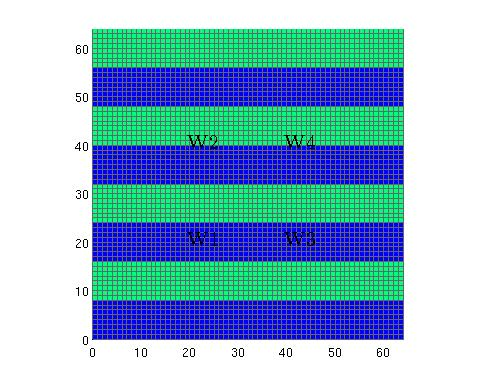
\includegraphics[width=4.3cm,height=4.3cm,keepaspectratio]{perm_he_1.jpg}
 \vspace{-20pt}
\caption{ Heterogeneous permeability, 4 wells.}\label{fig:hep}
\vspace{-15pt}
\end{wrapfigure}

\normalsize
As mentioned above, we studied flow through a porous medium with \emph{heterogeneous permeability} layers. A grid of
$nx = ny = 64$ elements is studied. We use 8 layers of the same size, 
4 layers with one value of permeability $\sigma_1$, followed by a layer with a different permeability value $\sigma_2$. Figure \ref{fig:hep} shows these layers. The permeability of one set of layers is set to $\sigma_1=1mD$, the permeability of the other set $\sigma_2$ is changed. 
Therefore, the contrast in permeability between the layers $(\frac{\sigma_2}{\sigma_1}=\sigma_2)$,
depends on the value of $\sigma_2$.\\
We investigate the dependence on the contrast in permeability value between the layers for the ICCG and DICCG methods.
The permeability  $\sigma_2$ varies from $\sigma_2=10^{-1}mD$ to $\sigma_2=10^{-3}mD$. 
 The tolerance is set as $10^{-11}$ for the snapshots as well as for the original problem.\\
\renewcommand{\arraystretch}{1.3}
\begin{table}[!ht]
\centering
\begin{minipage}{.65\textwidth}
\vspace{-20pt}
\centering
\begin{tabular}{ |c|c|c|c|} 
\hline
 $\kappa_2$ (mD) & $10^{-1}$& $10^{-2}$ & $10^{-3}$ \\
 \hline
  ICCG  & 75& 103&110\\ 
 
  DICCG  & 1 & 1& 1\\ 
 \hline
\end{tabular}
\caption{Table with the number of iterations for different contrasts in the permeability of the layers
for the ICCG and DICCG methods.}
\label{table:hei}\end{minipage}
\vspace{-10pt}
\end{table}

Table \ref{table:hei} shows the number of iterations required to achieve convergence 
for ICCG and DICCG for various permeability contrasts between the layers. \\
The plot of the residual and the solution 
to the problem are presented in Figures \ref{fig:convhe1} and \ref{fig:solhe1} for a value of permeability $\sigma_2=10^{-2}$.\\
In Table \ref{table:hei} we observe that the number of 
iterations increases when the contrast between the permeability layers increases for ICCG. For DICCG, 
we observe that we only need one iteration despite the change in permeability contrast between the layers.
\begin{figure}[!h]
\centering
\begin{minipage}{.4\textwidth}
 \centering
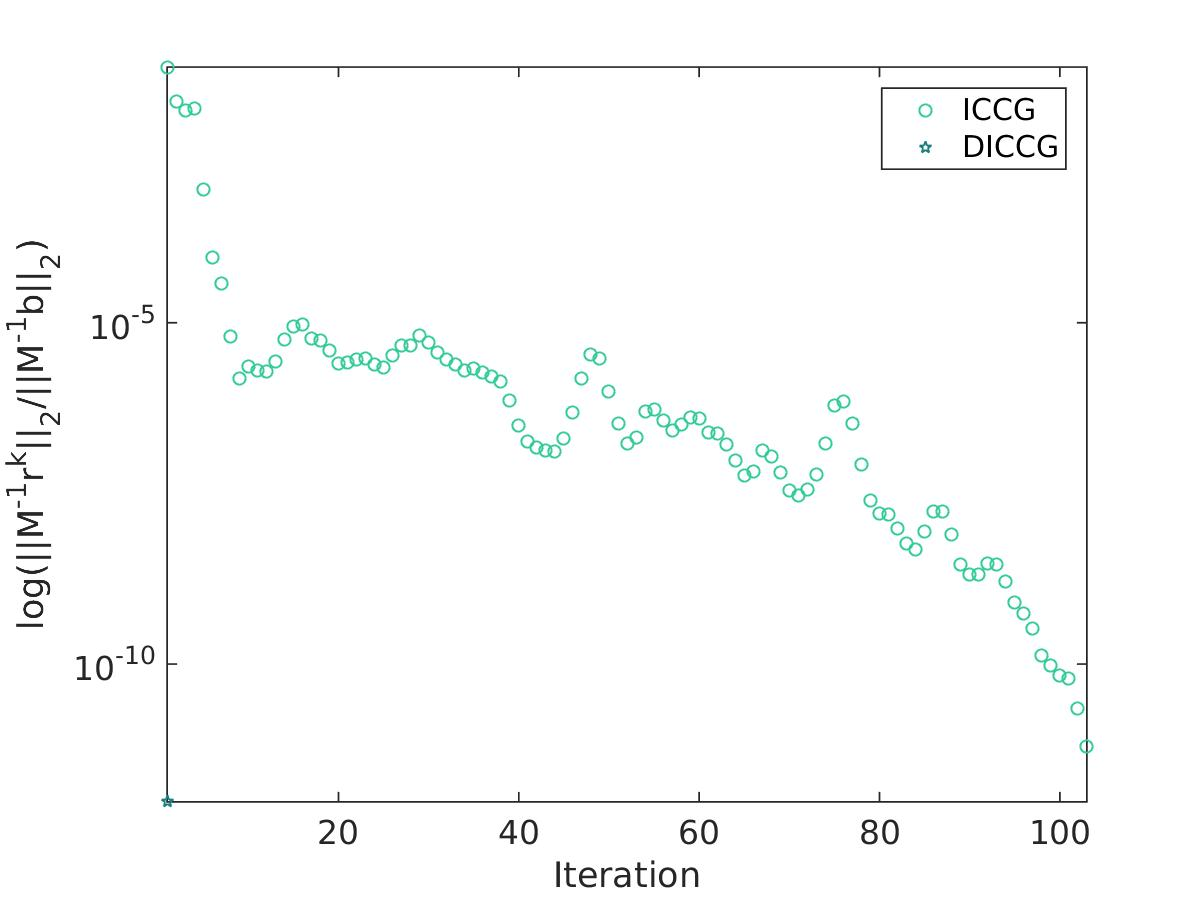
\includegraphics[width=5cm,height=5cm,keepaspectratio]
{conv_4w.jpg}
\caption{Convergence for the heterogeneous problem, 64 x 64 grid cells,  $\sigma_2=10^{-2}mD$.}
\label{fig:convhe1}
\end{minipage}%
\hspace{10pt}
\begin{minipage}{.4\textwidth} 
\centering 
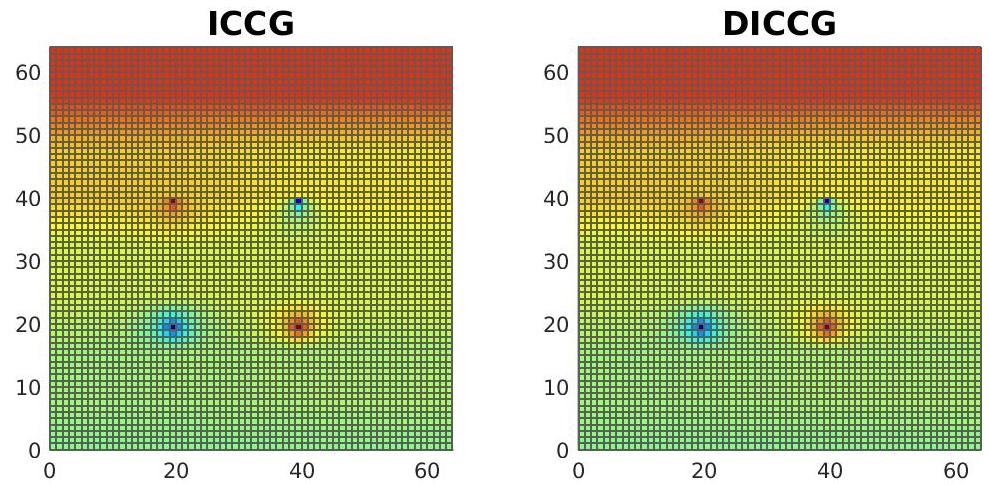
\includegraphics[width=6.5cm,height=6.5cm,keepaspectratio]
{sol_4w.jpg}
\caption{Solution of the heterogeneous problem, 64 x 64 grid cells, $\sigma_2=10^{-2}mD$.}
\label{fig:solhe1}
\end{minipage}
\end{figure}
%\begin{figure}[!h]
%\centering 
%\includegraphics[width=5cm,height=5cm,keepaspectratio]
%{perm_he_1.jpg}



\textbf{\emph{Case 2, Neumann boundary conditions everywhere.}}\\
In this case, four wells are positioned in the corners and have a bhp of -1 bar. One well
is positioned in the center of the domain and has a bhp of +4 bars
(see Figure \ref{fig:hep_2}). Homogeneous Neumann boundary conditions are posed on all boundaries. For this case, we use a set of four linearly independent snapshots as deflation vectors. We also use a linearly dependent set of 15 snapshots and the basis of POD (linearly independent set) obtained from the 15 snapshots. We set the same boundary conditions as in the original problem for all the snapshots.
The four linearly independent snapshots ($z_1-z_4$) are obtained giving a value of zero to one well and non-zero values to the other wells, such that the sum of the well pressures is equal to zero. The set of 15 snapshots are all the possible combinations of wells that satisfy that the flow in equals the flow out of the reservoir.
A summary of the configurations is presented below.
\renewcommand{\arraystretch}{1.3}
\begin{table}[!ht]\centering
\begin{minipage}{.45\textwidth}
\vspace{-10pt}
\centering
\begin{tabular}{ |c|c|c|c|c|c|} 
 \hline
  \multicolumn{6}{|l|}{System configuration} \\ 
  \hline
  \multicolumn{6}{|c|}{Well pressures (bars)}\\
  \hline
  &$W1$ &$W2$ &$W3$ &$W4$ &$W5$ \\
  \hline
&-1 & -1& -1& -1& -1\\
\hline
\multicolumn{6}{|l|}{Snapshots (4 linearly independent)} \\
\hline
 &$W1$ &$W2$ &$W3$ &$W4$ &$W5$ \\
  \hline

$\mathbf{z}_1$& 0&-1 &-1 &-1 &3 \\
$\mathbf{z}_2$& -1&0 &-1 &-1 &3  \\
$\mathbf{z}_3$& -1&-1 &0 &-1 &3  \\
$\mathbf{z}_4$& -1&-1 &-1 &0 &3  \\
 \hline
 \end{tabular}
\label{table:case2}\end{minipage}%
\hspace{10pt}
 \begin{minipage}{.45\textwidth}
 \begin{tabular}{ |c|c|c|c|c|c|} 
 \hline
 \multicolumn{6}{|l|}{Snapshots (linearly dependent)} \\
\hline
 &W1 &W2 &W3 &W4 &W5 \\
  \hline
$\mathbf{z}_5$& -1&-1 &-1 &-1 &4  \\
$\mathbf{z}_6$& -1&0 &0 &-1 &2  \\
$\mathbf{z}_7$& -1&-1 &0 &0 &2  \\
$\mathbf{z}_8$& -1&0 &-1 &0 &2  \\
$\mathbf{z}_9$& 0&-1 &-1 &0 &2  \\
$\mathbf{z}_{10}$& 0&-1 &0 &-1 &2  \\
$\mathbf{z}_{11}$& 0&0 &-1 &-1 &2  \\
$\mathbf{z}_{12}$& -1&0 &0 &0 &1  \\
$\mathbf{z}_{13}$& 0&-1 &0 &0 &1  \\
$\mathbf{z}_{14}$& 0&0 &-1 &0 &1  \\
$\mathbf{z}_{15}$& 0&0 &0 &-1 &1  \\
 \hline
 \end{tabular}

\label{table:case2}\end{minipage}\caption{Table with the well configuration of the system and the snapshots used for the Case 2, we use homogeneous Neumann boundary conditions.}
\vspace{-10pt}
\end{table}

\normalsize

\emph{Heterogeneous permeability layers}\\

\begin{wrapfigure}{R}{4.3cm}
\centering 
\vspace{-10pt}
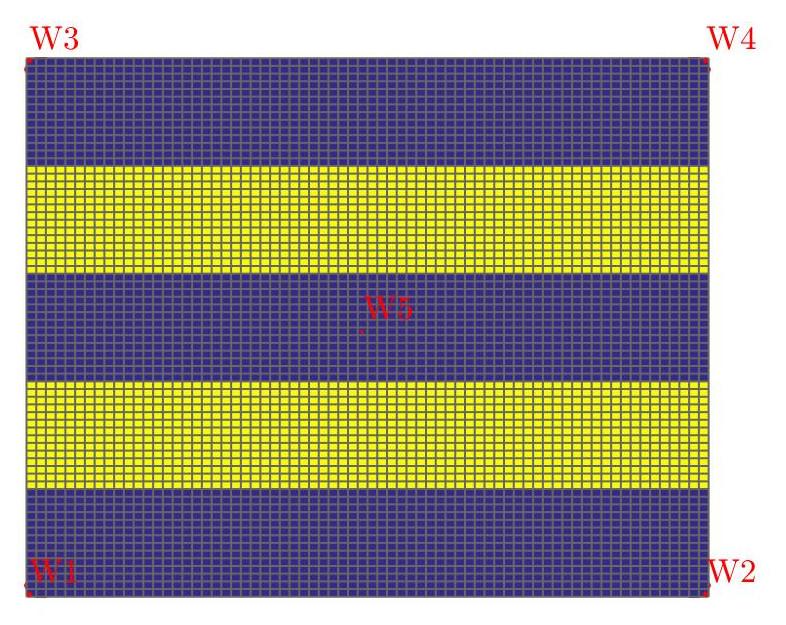
\includegraphics[width=4.7cm,height=4.7cm,keepaspectratio]{/mnt/sda2/cortes/Results/sp_article/Incompressible/size_64perm_2_5wells11/perm.jpg}
 \vspace{-25pt}
\caption{ Heterogeneous permeability, 5 wells.}\label{fig:hep_2}
\vspace{-15pt}
\end{wrapfigure} 
As in the previous case, single-phase flow through a porous medium with heterogeneous permeability layers is studied.
A grid of $nx = ny = 64$ elements is investigated. The deflation vectors used in this case are the 4 snapshots ($\mathbf{z}_1$-$\mathbf{z}_4$), a set of 15 linearly dependent vectors and 4 basis vectors obtained for the POD method from the latter set.\\
The snapshots and the solutions are obtained with a tolerance of $10^{-11}$. \\
\begin{figure}[!ht]
%\begin{wrapfigure}{R}{5cm}
%\vspace{-20pt}
 \centering
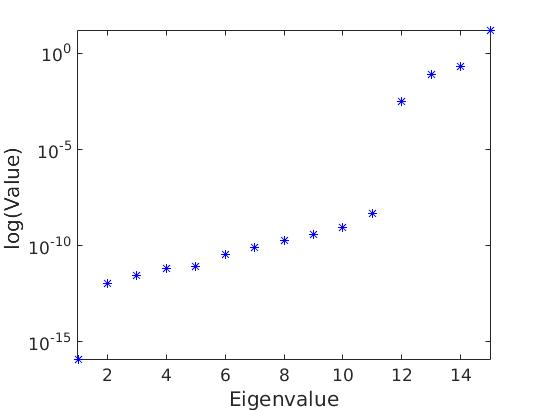
\includegraphics[width=7cm,height=7cm,keepaspectratio]
{/mnt/sda2/cortes/Results/sp_article/Incompressible/size_64perm_2_5wells11/eig_pod.jpg}
%\vspace{-10pt}
\caption{Eigenvalues of the snapshot correlation matrix $\mathbf{R}=\mathbf{X}\mathbf{X}^T$, if 15 snapshots are used.}
%\vspace{-20pt}
\label{fig:eig}
%\end{wrapfigure}
\end{figure} 
Table \ref{table:he22} shows the number of iterations required to reach convergence for the ICCG method and the deflation method with four linearly independent snapshots as deflation vectors DICCG$_{4}$, 15 linearly dependent snapshots DICCG$_{15}$ and the basis vectors of POD, DICC$G_{POD}$\footnote{The * means that the solution is not reached.}. 
For the deflation vectors of DICCG$_{POD}$ we plot the eigenvalues of the snapshot correlation matrix $\mathbf{R}=\mathbf{X}^T \mathbf{X}$ (see section \ref{POD}) in Figure \ref{fig:eig}. We observe that there are 4 eigenvalues much larger than the rest of the eigenvalues which are responsible for the divergence of the method. In DICCG$_{POD}$ we use the eigenvectors corresponding to the larger eigenvalues as deflation vectors.\\
The plot of the residual and the solution of the problem are presented in
Figure \ref{fig:convhe2} and \ref{fig:solhe2} for the ICCG and DICCG methods for the case of $\sigma_2=10^{-2}$.\\
\renewcommand{\arraystretch}{1.3}
\begin{table}[!ht]\centering
\begin{minipage}{.8\textwidth}
\vspace{-10pt}
\centering
\begin{tabular}{ |c|c|c|c|} 
\hline
 $\sigma_2$ (mD) & $10^{-1}$& $10^{-2}$ & $10^{-3}$ \\
 \hline
  ICCG  & 90& 115&131\\ 
 
  DICCG$_4$  & 1 & 1& 1\\ 
  DICCG$_{15}$  & 200* & 200*& 200*\\
  DICCG$_{POD}$  & 1 & 1& 1\\
 \hline
\end{tabular}
\caption{Table with the number of iterations for different contrast in the permeability of the layers
for the ICCG, DICCG$_4$, DICCG$_{15}$, and DICCG$_{POD}$ methods, tolerance of solvers and snapshots $10^{-11}$.}
\label{table:he22}\end{minipage}
\vspace{-10pt}
\end{table}

In Table \ref{table:he22}, for the ICCG method, we observe that the number of iterations 
increases if the contrast in the permeability increases. For the DICCG method with 4 linearly independent deflation vectors and 4 basis vectors of POD, convergence is reached 
within one iteration. However, for the case of 15 linearly dependent vectors, the solution is not reached within the 200 iterations allowed for this problem.\\

\vspace{-5mm}
\begin{figure}[!h]
\centering
\begin{minipage}{.4\textwidth}
 \centering
\includegraphics[width=6.5cm,height=6.5cm,keepaspectratio]
{/mnt/sda2/cortes/Results/sp_article/Incompressible/size_64perm_2_5wells11/conv_deftol-11.jpg}
\caption{Convergence for the heterogeneous problem, 64 x 64 grid cells, $\sigma_2=10^{-2}$.}
\label{fig:convhe2}
\end{minipage}%
\hspace{10 pt}
\begin{minipage}{.4\textwidth}
 \centering
 %\vspace{-2cm}
\includegraphics[width=4cm,height=4cm,keepaspectratio]
{/mnt/sda2/cortes/Results/sp_article/Incompressible/size_64perm_2_5wells11/solpodtol-11.jpg}
\vspace{0.5cm}
\caption{Solution of the heterogeneous problem, 64 x 64 grid cells, $\sigma_2=10^{-2}$.}
\label{fig:solhe2}
\end{minipage}
\end{figure}

\newpage
\emph{SPE 10 model}\\
This model has large variations in the permeability coefficients, the contrast between coefficients is of the order of $ 10^7$.
It has 5 sources or wells, four producers in the corners (negative) and one injector in the center (positive).
The model contains 60 x 220 x 85 cells. We study the dependence of the ICCG and the DICCG method on the size of the problem. One layer is studied with various grid sizes 16 x 56, 30 x 110, 46 x 166 and 60 x 220, and the complete model containing 85 layers.
Permeability is upscaled
averaging the permeability in each grid using the harmonic-arithmetic average algorithm from MRST.
The permeability of the coarser grid (16 x 56 cells) is shown in Figure \ref{fig:permc} and the complete model in Figure \ref{fig:permcc}.
The permeability contrast for the diverse grid size problems is shown in Table \ref{table:permgs}. From this table, we observe that the contrast in the permeability for different grid sizes varies slightly, but that the order
of magnitude remains the same for all the cases.\\
Snapshots are obtained solving the system with different well
configurations (\emph{Configuration 2}). As before, we simulate single-phase incompressible flow.\\
The system and snapshots are solved with an accuracy of $10^{-11}$.
In the first experiment with the deflation method, the four linearly independent snapshots are used as deflation vectors (DICCG). Then, 
15 linearly dependent vectors and finally 4 vectors of the POD basis are used as deflation vectors (DICCG$_{POD}$). \\ 
\begin{figure}[!h]
\centering
\begin{minipage}{.4\textwidth}
 \centering
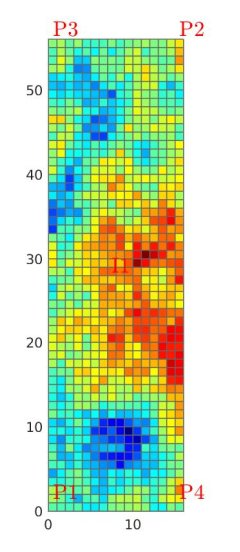
\includegraphics[width=4.5cm,height=4.5cm,keepaspectratio]
{perm_layer_2.jpg}
\caption{SPE 10 benchmark, 2nd layer 16 x 56 grid cells, permeability field.}
\label{fig:permc}
\end{minipage}%
\hspace{4mm}
\begin{minipage}{.4\textwidth}
 \centering
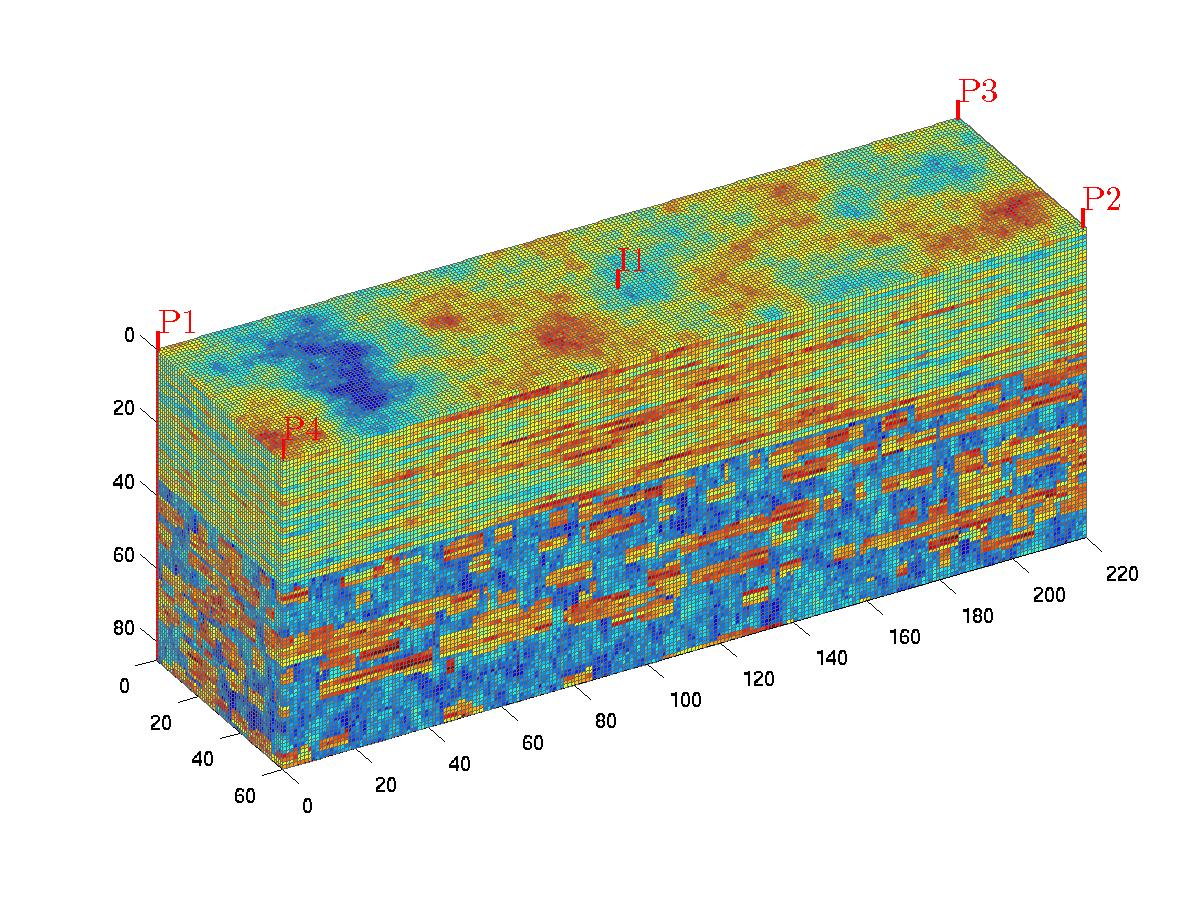
\includegraphics[width=5.5cm,height=5.5cm,keepaspectratio]
{perm_layer_.jpg}
\caption{SPE 10 benchmark, permeability field.}
\label{fig:permcc}
\end{minipage}
\end{figure}


\begin{table}[!ht]
\centering
\begin{tabular}{ |c|c|c|c|c|c|  } 
 \hline
  Grid size & 16x56x1& 30x110x1& 46x166x1& 60x220x1&60x220x85\\
  \hline
  Contrast ($\times10^{7}$) & 1.04 & 2.52&  2.6&  2.8 &3\\ 
\hline
\end{tabular}
\caption{Table with the number of iterations for different grid sizes
for the ICCG, DICCG$_4$, DICCG$_{15}$, and DICCG$_{POD}$ methods, tolerance of solvers and snapshots $10^{-11}$.}
\label{table:permgs}
\end{table}

The number of iterations required to achieve convergence with the ICCG and DICCG methods for various grid sizes is presented in Table \ref{table:itgrid}. \\
The convergence and the solution obtained with the ICCG and DICCG methods are presented in Figure \ref{fig:convspe85} and Figure \ref{fig:solspe} for the complete problem. 
In Table \ref{table:itgrid} we observe that for the ICCG method the required iterations to reach convergence increases as the size of the grid increases. Meanwhile, for the deflated methods only few iterations are required and it does not depend on the size of the grid. The large contrast in the permeability field may require higher accuracy in the snapshots to find the solution with a deflated method within one iteration (see \cite{Diaz16}) within the imposed tolerance. However, we observe in Figure \ref{fig:convspe85} that the first iteration has a relative residual smaller than $10^{-10}$ for the DICCG$_4$ and DICCG$_{POD}$ methods.
We also observe that for the deflated method with 15 linearly dependent snapshots as deflation vectors (DICCG$_{15}$), the relative residual is close to $10^{-7}$ for the first time steps, and then it increases, which shows that this choice leads to a inestable method (note that the matrix $E$ is a nearly singular matrix). 

\begin{table}[!ht]
\centering
\begin{tabular}{|c |c|c|c|c|c| c| } 
 \hline
Method  & 16x56x1& 30x110x1& 46x166x1& 60x220x1&60x220x85\\
   \hline
  ICCG & 45 & 101&  178 &  219&1011 \\ 
   DICCG$_{15}$ & 500* & 500*&  500* &  500*& 2000*\\ 
   DICCG$_{4}$ & 1 & 2&  3 &  2& 2\\  
   DICCG$_{POD}$ & 1 & 2&  3 &  2 &2\\ 
\hline
\end{tabular}
\caption{Table with the number of iterations for ICCG and DICCG methods, 
various grid sizes.}
\label{table:itgrid}
\end{table}

\begin{figure}[!h]
\centering
\begin{minipage}{.5\textwidth}
 \centering
\includegraphics[width=7cm,height=7cm,keepaspectratio]
{/mnt/sda2/cortes/Results/16_09/article_sp/SPE10_85layers_5w_tol-11/conv_deftol-11.jpg}
\caption{Convergence for the SPE 10 benchmark, 60 x 220 x 85 grid cells, accuracy of the snapshots and solvers $10 ^{-11}$.}
\label{fig:convspe85}
\end{minipage}%
\hspace{3mm}
\begin{minipage}{.45\textwidth}
 \centering
\includegraphics[width=6cm,height=6cm,keepaspectratio]
{/mnt/sda2/cortes/Results/16_09/article_sp/SPE10_85layers_5w_tol-11/solution.jpg}
\vspace{.7cm}
\caption{Solution of the SPE 10 benchmark, 60 x 220 x 85 grid cells, accuracy of the snapshots and solvers $10 ^{-11}$.}
\label{fig:solspe}
\end{minipage}
\end{figure}
\newpage

\newpage
\newpage
\subsection{Compressible Problem}
\emph{\textbf{Model parameters}}\\

In this section we model single-phase flow through a porous medium for a case when the density depends on the pressure 
according to Equation \ref{eq:rhoeq}. We solve Equation \eqref{eq:ce6} for a fluid with the following characteristics:
\begin{itemize}
 \item $\mu = 1 cp$,
 \item $\rho = 1014 kg/m^3$,
\end{itemize}
In the compressible case, the compressibility of the fluid is:
\begin{itemize}
 \item $c= 1 \times 10^{-3}$.
\end{itemize}
Equation \eqref{eq:ce6} is non-linear due to the dependence of the density on the pressure. Therefore, we need to 
linearize this equation via the Newton-Raphson method and solve the resulting linear system. After linearization we obtain the linear system \eqref{eq:lsJ} and we solve it with an iterative method, a summary of the procedure is presented in Table \ref{table:solstages}. The simulation, with exception of the linear solvers, is performed with MRST. Automatic Differentiation (AD) is used for the NR loop \cite{Lie13}. The resulting linear system is solved with ICCG and DICCG methods. We compute the solution of the system for the first 10 time steps with the ICCG method. The rest of the time steps is solved with DICCG, using as deflation vectors POD basis vectors computed from the solution of the ten previous time steps. The number of deflation vectors are specified in each problem. \\
\begin{wrapfigure}{R}{5cm}
\centering 
\vspace{-20pt}
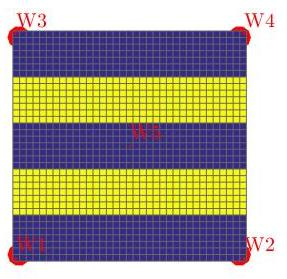
\includegraphics[width=5cm,height=5cm,keepaspectratio]{perm_comp.jpg}
 \vspace{-15pt}
\caption{ Heterogeneous permeability, 5 wells, compressible problem.}\label{fig:pc}
\vspace{-10pt}
\end{wrapfigure} 

We study an academic layered problem that consists of layers with two different permeability values 
(see Figure \ref{fig:pc}). The first layer has a permeability of $\sigma_1 = 30mD$, and the permeability 
of the second layer is varied $\sigma_2 =$ [3mD, 0.3mD, 0.03mD]. Therefore, the contrast between the layers 
is $10^{-1},$ $10^{-2}$ and $10^{-3}$.
The domain is a square with five wells, Four of which are positioned in the corners of the domain and one 
well is placed in the center. The length of the domain is 70 m and three different grid sizes are studied: 
35, 70 and 105 grid cells in each dimension.  We use homogeneous Neumann boundary conditions on all boundaries. \\
The initial pressure of the reservoir is set as 200 bars. The pressure in the corner wells is 100 bars and 
in the central well is 600 bars.  
%A summary of the well configuration is presented in Table \ref{table:ccase1}.\\
%  \renewcommand{\arraystretch}{1.3}
% \begin{table}[!ht]\centering
% \begin{minipage}{.7\textwidth}
% \vspace{-10pt}
% \centering
% \begin{tabular}{ |c|c|c|c|c|c|} 
%  \hline
%   \multicolumn{6}{|l|}{System configuration} \\ 
%   \hline
%   \multicolumn{6}{|c|}{Well pressures (bars)}\\
%   \hline
%   &W1 &W2 &W3 &W4 &W5 \\
%   \hline
% &100 & 100& 100& 100& 600\\
% \hline
% \multicolumn{6}{|l|}{Snapshots } \\
%   \hline
% $\mathbf{z}_1$&200 & 100& 100& 100& 500\\
% $\mathbf{z}_2$&100 & 200& 100& 100& 500\\
% $\mathbf{z}_3$&100 & 100& 200& 100& 500\\
% $\mathbf{z}_4$&100 & 100& 100& 200& 500\\
%  \hline
%  \end{tabular}
% \caption{Table with the well configuration of the system and the snapshots used for the compressible problem Case 1, we use homogeneous Neumann boundary conditions.}\label{table:ccase1}
% \end{minipage}
% \end{table}
The simulation was performed during 152 days with 52 time steps and a time step of 3 days. The tolerance of 
the NR method and the linear solvers is $10^{-5}$.\\
\newpage
\textbf{Different contrast in permeability.}\\
As mentioned previously we change the contrast between the permeability layers, in this section we present 
the results obtained for three different contrast for a 2D Cartesian grid of $35 \times 35$ grid cells covering 
an area of $70 \times 70$ m$^2$. As a first set of experiments, we compute 10 snapshots, solutions to the first 
10 time steps, with ICCG and we use these snapshots as deflation vectors to solve the rest of the time steps with 
deflation DICCG$_{10}$. After the first thes snapshots are computed, we update the snapshots with the most recently 
computed solution, such that the ten snapshots correspond to the ten solutions of the ten previous time steps. 
We compute SVD of the matrix constructed with these snapshots as columns and we study the eigenvalues obtained 
to select as deflation vectors the eigenvectors corresponding to the largest eigenvalues. 

\textbf{Contrast between permeability layers of $10^{-1}$.}\\
In Figure \ref{fig:compsol_1}, the solution obtained with the ICCG method is presented, the solution is the same 
for all methods. The upper left figure represents the pressure field at the final time step. The upper right 
figure represents the pressure across the diagonal joining the (0,0) and (35,35) grid cells for all the time steps. 
We observe the initial pressure (200 bars) across this diagonal and the evolution of the pressure field through time. 
In the lower figure, we observe the surface volume rate for the five wells during the simulation.

\begin{figure}[!h]
\centering
\begin{minipage}{.7\textwidth}
 \centering
\includegraphics[width=8cm,height=8cm,keepaspectratio]
{/home/wagm/cortes/Localdisk/Results/sp_article/10_13/size_35perm_1_5wells_c_1e-3_s_52upd/solution.jpg}
\caption{Solution of the compressible problem solved with the ICCG method for a layered problem with a contrast between permeability layers of $10^{-1}$ in a domain of $70 \times 70$ m$^2$.}
\label{fig:compsol_1}
\end{minipage}
\end{figure}

As a second set of experiments, we use basis vectors of POD as deflation vectors of the DICCG method, these basis vectors are the eigenvectors corresponding of the largest eigenvalues of the snapshot correlation matrix $\mathbf{X}$ (see Section \ref{POD}). The snapshot correlation matrix is constructed with the previously computed solutions, i.e., the solutions of the previous time steps. As mentioned before, for each time step, the previous 10 solutions are used as snapshots to compute the POD basis. The eigenvalues of the snapshot correlation matrix $\mathbf{R}=\frac{1}{m}\mathbf{X}\mathbf{X}^T$ constructed with the previous ten time steps are presented in Figure \ref{fig:eig_POD_1} for the 20$^{th}$ time step. In this figure, we observe that six eigenvalues are larger than the rest. Therefore, we use the eigenvectors corresponding to these six eigenvalues as deflation vectors (DICCG$_6$). 
\begin{figure}[!h]
\centering
\begin{minipage}{.4\textwidth}
 \centering
 \vspace{-3mm}
\includegraphics[width=6cm,height=6cm,keepaspectratio]{/home/wagm/cortes/Localdisk/Results/sp_article/10_13/lenght_70size_35/perm_1_5wells_c_1e-3_s_52upddv_10/eigs/eigs1stepA.jpg}
 \vspace{-10pt}
\caption{Eigenvalues of the original matrix $\mathbf{J}$, time step 1 for a layered problem with a contrast between permeability layers of $10^{-1}$ in a domain of $70 \times 70$ m$^2$.}\label{fig:eigs_A_1}
\end{minipage}%
\hspace{1cm}
\begin{minipage}{.4\textwidth}
 \centering
 %\vspace{-5mm}
\includegraphics[width=6cm,height=6cm,keepaspectratio]{/home/wagm/cortes/Localdisk/Results/sp_article/10_13/lenght_70size_35/perm_1_5wells_c_1e-3_s_52upddv_10pod5-10/eig_pod20.jpg}
\vspace{-5mm}
\caption{Eigenvalues of the data snapshot correlation matrix $\mathbf{R}=\mathbf{X}\mathbf{X}^T$, time step 20 for a layered problem with a contrast between permeability layers of $10^{-1}$ in a domain of $70 \times 70$ m$^2$.}
\label{fig:eig_POD_1}
\end{minipage}
\end{figure}

For this problem, only the first time step requires more than two NR iterations. Therefore, we solely study the 
behavior of the linear solvers during the first two NR iterations. The number of iterations necessary to reach 
convergence with the linear solvers is presented for the first two NR iterations in Figure \ref{fig:NR_IC_1} 
for the ICCG method, Figure \ref{fig:NR_D10_1} for the deflated method DICCG$_{10}$ using 10 snapshots as 
deflation vectors and Figure \ref{fig:NR_D6_1} using 6 POD basis vectors as deflation vectors.
The eigenvalues of the matrices are presented in Figure \ref{fig:eigs_A_1} for the original system matrix 
$\mathbf{J}$ for the first time step, Figure \ref{fig:eigs_MA_1} for the preconditioned system, Figure 
\ref{fig:eigs_PA10_1} for DICCG$_{10}$ and Figure \ref{fig:eigs_PA6_1} the deflated system DICCG$_6$. 
The preconditioned system is studied for the first time step, and the deflated systems are studied for the 11$^{th}$ 
time step. For the preconditioned and the deflated system, the same scale is used for the comparison.\\

%The eigenvalues of the covariance matrix  $\bar{\mathbf{R}}=\frac{1}{m}\sum_{i=1}^{m}(\mathbf{z}_i-\mathbf{z})(\mathbf{z}_i-\mathbf{z})^T$ are presented in Figure \ref{fig:eig_PODr}.\\

\begin{figure}[!h]
\centering
\begin{minipage}{.4\textwidth}
\vspace{-0.9cm}
\hspace{-1cm}
\includegraphics[width=8cm,height=8cm,keepaspectratio]
{/home/wagm/cortes/Localdisk/Results/sp_article/10_13/lenght_70size_35/perm_1_5wells_c_1e-3_s_52upd/iterations_4NR.jpg}
\vspace{-1.3cm}
\caption{Number of iterations of the ICCG method for the first two NR iterations for a layered problem with a contrast between permeability layers of $10^{-1}$ in a domain of $70 \times 70$ m$^2$.}
\label{fig:NR_IC_1}
\end{minipage}%
\hspace{15mm}
\begin{minipage}{.4\textwidth}
 \centering
 \vspace{-5mm}
\includegraphics[width=6cm,height=6cm,keepaspectratio]
{/home/wagm/cortes/Localdisk/Results/sp_article/10_13/lenght_70size_35/perm_1_5wells_c_1e-3_s_52upd/eigs/eigs1step.jpg}
\caption{Eigenvalues of the preconditioned matrix, time step for a layered problem with a contrast between permeability layers of $10^{-1}$ in a domain of $70 \times 70$ m$^2$.}
\label{fig:eigs_MA_1}
\end{minipage}
\end{figure}



\begin{figure}[!h]
\centering
\begin{minipage}{.4\textwidth}
\vspace{-0.4cm}
\hspace{-1cm}
\includegraphics[width=8cm,height=8cm,keepaspectratio]
{/home/wagm/cortes/Localdisk/Results/sp_article/10_16/lenght_70size_35/perm_2_5wells_c_1e-3_s_52upddv_10/iterations_4NR.jpg}
\vspace{-1.3cm}
\caption{Number of iterations of the DICCG$_{10}$ method for the first two NR iterations for a layered problem with a contrast between permeability layers of $10^{-1}$ in a domain of $70 \times 70$ m$^2$.}
\label{fig:NR_D10_1}
\end{minipage}%
\hspace{15mm}
\begin{minipage}{.4\textwidth}
 \centering
\includegraphics[width=6cm,height=6cm,keepaspectratio]
{/home/wagm/cortes/Localdisk/Results/sp_article/10_16/lenght_70size_35/perm_2_5wells_c_1e-3_s_52upddv_10/eigs/eigsPA11step.jpg}
\caption{Eigenvalues of the deflated system DICCG$_{10}$ for a layered problem with a contrast between permeability layers of $10^{-1}$ in a domain of $70 \times 70$ m$^2$.}
\label{fig:eigs_PA10_1}
\end{minipage}
\end{figure}



\begin{figure}[!h]
\centering
\begin{minipage}{.4\textwidth}
\vspace{-0.4cm}
\hspace{-1cm}
\includegraphics[width=8cm,height=8cm,keepaspectratio]
{/home/wagm/cortes/Localdisk/Results/sp_article/10_13/lenght_70size_35/perm_1_5wells_c_1e-3_s_52upddv_10pod5-10/iterations_4NR.jpg}
\vspace{-1.3cm}
\caption{Number of iterations of the DICCG$_6$ method for the first two NR iterations for a layered problem with a contrast between permeability layers of $10^{-1}$ in a domain of $70 \times 70$ m$^2$.}
\label{fig:NR_D6_1}
\end{minipage}%
\hspace{15mm}
\begin{minipage}{.4\textwidth}
 \centering
\includegraphics[width=6cm,height=6cm,keepaspectratio]
{/home/wagm/cortes/Localdisk/Results/sp_article/10_13/lenght_70size_35/perm_1_5wells_c_1e-3_s_52upddv_10pod5-10/eigs/eigsPA11step.jpg}
\caption{Eigenvalues of the deflated system DICCG$_6$ for a layered problem with a contrast between permeability layers of $10^{-1}$ in a domain of $70 \times 70$ m$^2$.}
\label{fig:eigs_PA6_1}
\end{minipage}
\end{figure}

From Figure \ref{fig:eigs_MA_1}, Figure \ref{fig:eigs_PA10_1} and Figure \ref{fig:eigs_PA6_1} we observe that the smallest eigenvalues are not longer visible in the system. This is because we use the same scale for the plots in all the figures and with the deflation methods we remove the smallest eigenvalues, they are sent to zero, in this case to a very small value. As they are very small, they are not longer important for the convergence of the system. After removing these eigenvalues, the condition number is reduced and therefore we obtain an acceleration in the convergence of the method (see Section \ref{def}). From the spectrum of these systems, we observe that after the deflation procedure we reduce in one order of magnitude the condition number (see Table \ref{table:cn_1}), the order the magnitude of the eigenvalues is the same for both deflation cases (10 and 6 deflation vectors).\\

\begin{table}[!ht]\centering
\begin{minipage}{.7\textwidth}
\vspace{-10pt}
\centering
\begin{tabular}{ |c|c|c|c|} 
  \hline
 Matrix &$\lambda_{max}$ &$\lambda_{min}$ &$\kappa_2=\frac{\lambda_{max}}{\lambda_{min}}$  \\
  \hline
$\mathbf{M}^{-1}\mathbf{J}$ &1 & $\approx 10^{-2}$&$\approx 10^2$\\
$\mathbf{P}\mathbf{M}^{-1}\mathbf{J}$ &1 & $\approx 10^{-1}$&$\approx 10^1$\\
 \hline
 \end{tabular}
\caption{Condition number of the preconditioned and deflated systems for a layered problem with a contrast between permeability layers of $10^{-1}$ in a domain of $70 \times 70$ m$^2$.}\label{table:cn_1}
\end{minipage}
\end{table}

From Figure \ref{fig:NR_IC_1},  Figure \ref{fig:NR_D10_1} and Figure \ref{fig:NR_D6_1}, we observe that the reduction of the condition number results in a reduction of the number of iterations for the first and second NR iterations of the deflated methods (DICCG$_{10}$, DICCG$_6$) compared with the ICCG method. For the ICCG method, we need on average 15 and 19 linear iterations in the first two NR iterations to reach the desired tolerance. In contrast, for the deflated methods, we need on average 1 or 2 linear iterations for the first NR iteration. For the second NR iteration, after the computation of the snapshots, instead of computing the solution for all the remaining 42 time steps computed for the ICCG method, we only need to compute 18 times steps with an average of 3 and 11 linear iterations. Which implies that the convergence is already achieved after the first NR iteration for the rest of the time steps. A summary of the average number of iterations is presented in Table \ref{table:liter1} and Table \
ref{table:liter2}.\\

 
\textbf{Contrast between permeability layers of $10^{-2}$.}\\
We repeat the experiments of previous sections. In this case, the contrast between permeability layers is $10^{-2}$. 
The solution obtained with the ICCG method is presented in Figure \ref{fig:compsol_2}, the solution is the same 
for the DICCG method. The eigenvalues of the snapshot correlation matrix $\mathbf{R}$ for the 20$^{th}$ time 
step are presented in Figure \ref{fig:eig_POD_2}. 
From this figure, we observe that there are 7 eigenvalues of the correlation matrix larger than the rest. 
Therefore, the largest amount of information might be contained in these vectors. For this problem, we studied 
the deflation method using 6 (DICCG$_6$) and 7 (DICCG$_7$) POD basis vectors as deflation vectors as well as 
the DICCG$_{10}$ method with 10 snapshots as deflation vectors. 

\begin{figure}[!h]
\centering
\begin{minipage}{.7\textwidth}
 \centering
\includegraphics[width=8cm,height=8cm,keepaspectratio]
{/home/wagm/cortes/Localdisk/Results/sp_article/10_13/lenght_70size_35/perm_2_5wells_c_1e-3_s_52upddv_10pod5-10/solution.jpg}
\caption{Solution of the compressible problem solved with the ICCG method for a layered problem with a contrast between permeability layers of $10^{-2}$ in a domain of $70 \times 70$ m$^2$.}
\label{fig:compsol_2}
\end{minipage}
\end{figure}

\begin{figure}[!h]
\centering
\begin{minipage}{.4\textwidth}
 \centering
 \vspace{-3mm}
\includegraphics[width=6cm,height=6cm,keepaspectratio]{/home/wagm/cortes/Localdisk/Results/sp_article/10_13/lenght_70size_35/perm_2_5wells_c_1e-3_s_52upddv_10pod5-10/eigs/eigs1stepA.jpg}
 \vspace{-10pt}
\caption{Eigenvalues of the original matrix $\mathbf{J}$, time step 1 for a layered problem with a contrast between permeability layers of $10^{-2}$ in a domain of $70 \times 70$ m$^2$.}\label{fig:eigs_A_2}
\end{minipage}%
\hspace{1cm}
\begin{minipage}{.4\textwidth}
 \centering
 %\vspace{-5mm}
\includegraphics[width=6cm,height=6cm,keepaspectratio]{/home/wagm/cortes/Localdisk/Results/sp_article/10_13/lenght_70size_35/perm_2_5wells_c_1e-3_s_52upddv_10pod5-10/eig_pod20.jpg}
\vspace{-5mm}
\caption{Eigenvalues of the data snapshot correlation matrix $\mathbf{R}=\mathbf{X}\mathbf{X}^T$, time step 20 for a layered problem with a contrast between permeability layers of $10^{-2}$ in a domain of $70 \times 70$ m$^2$.}
\label{fig:eig_POD_2}
\end{minipage}
\end{figure}

%\begin{minipage}{1\textwidth}
As in the previous case, we study the behavior of the linear solvers only for the first two NR iterations. 
The number of iterations necessary to reach convergence with the linear solvers is presented for the first two 
NR iterations in Figure \ref{fig:NR_IC_2} for the ICCG method, Figure \ref{fig:NR_D10_2} for the deflated method 
DICCG$_{10}$, Figure \ref{fig:NR_D6_2} for DICCG$_6$ and Figure \ref{fig:NR_D7_2} for DICCG$_7$.
The eigenvalues of the matrices are presented in Figure \ref{fig:eigs_A_2} for the original system matrix $\mathbf{J}$ 
for the first time step, Figure \ref{fig:eigs_MA_2} for the preconditioned system,  Figure \ref{fig:eigs_PA10_2} 
the deflated system DICCG$_{10}$, Figure \ref{fig:eigs_PA6_2} the deflated system DICCG$_6$ and Figure 
\ref{fig:eigs_PA7_2} for DICCG$_7$. From the previously mentioned figures, we observe that some eigenvalues from 
the preconditioned system are not longer in the plot for deflated systems, this is because they are very small and 
they are not longer visible in the system. When we use 10 snapshots as deflation vectors, we remove more eigenvalues 
than when use 6 or 7, but the order of magnitude of the smallest eigenvalue is the the same for all cases, which 
means that the behavior should be similar. Comparing the cases when we have 6 and 7 deflation vectors, we observe 
that both spectra are almost the same except for one eigenvalue that is smaller than the case when we 
use 6 deflation vectors (Figure \ref{fig:eigs_PA6_2}). Hence, we expect a slightly better behavior when using 7 
deflation vectors. \\
%\end{minipage} 

\begin{figure}[!h]
\centering
\begin{minipage}{.4\textwidth}
\vspace{-0.9cm}
\hspace{-1cm}
\includegraphics[width=8cm,height=8cm,keepaspectratio]
{/home/wagm/cortes/Localdisk/Results/sp_article/10_13/lenght_70size_35/perm_2_5wells_c_1e-3_s_52upd/iterations_4NR.jpg}
\vspace{-1.3cm}
\caption{Number of iterations of the ICCG method for the first two NR iterations for a layered problem with a contrast between permeability layers of $10^{-2}$ in a domain of $70 \times 70$ m$^2$.}
\label{fig:NR_IC_2}
\end{minipage}%
\hspace{15mm}
\begin{minipage}{.4\textwidth}
 \centering
 \vspace{-5mm}
\includegraphics[width=6cm,height=6cm,keepaspectratio]
{/home/wagm/cortes/Localdisk/Results/sp_article/10_13/lenght_70size_35/perm_2_5wells_c_1e-3_s_52upd/eigs/eigs1step.jpg}
\caption{Eigenvalues of the preconditioned matrix, time step 1 for a layered problem with a contrast between permeability layers of $10^{-2}$ in a domain of $70 \times 70$ m$^2$.}
\label{fig:eigs_MA_2}
\end{minipage}
\end{figure}


\begin{figure}[!h]
\centering
\begin{minipage}{.4\textwidth}
\vspace{-0.4cm}
\hspace{-1cm}
\includegraphics[width=8cm,height=8cm,keepaspectratio]
{/home/wagm/cortes/Localdisk/Results/sp_article/10_16/lenght_70size_35/perm_2_5wells_c_1e-3_s_52upddv_10/iterations_4NR.jpg}
\vspace{-1.3cm}
\caption{Number of iterations of the DICCG$_{10}$ method for the first two NR iterations for a layered problem with a contrast between permeability layers of $10^{-2}$ in a domain of $70 \times 70$ m$^2$.}
\label{fig:NR_D10_2}
\end{minipage}%
\hspace{15mm}
\begin{minipage}{.4\textwidth}
 \centering
\includegraphics[width=6cm,height=6cm,keepaspectratio]
{/home/wagm/cortes/Localdisk/Results/sp_article/10_16/lenght_70size_35/perm_2_5wells_c_1e-3_s_52upddv_10/eigs/eigsPA11step.jpg}
\caption{Eigenvalues of the deflated system DICCG$_{10}$ for a layered problem with a contrast between permeability layers of $10^{-2}$ in a domain of $70 \times 70$ m$^2$.}
\label{fig:eigs_PA10_2}
\end{minipage}
\end{figure}


\begin{figure}[!h]
\centering
\begin{minipage}{.4\textwidth}
\vspace{-0.4cm}
\hspace{-1cm}
\includegraphics[width=8cm,height=8cm,keepaspectratio]
{/home/wagm/cortes/Localdisk/Results/sp_article/10_13/lenght_70size_35/perm_2_5wells_c_1e-3_s_52upddv_10pod5-10/iterations_4NR.jpg}
\vspace{-1.3cm}
\caption{Number of iterations of the DICCG$_6$ method for the first two NR iterations for a layered problem with a contrast between permeability layers of $10^{-2}$ in a domain of $70 \times 70$ m$^2$.}
\label{fig:NR_D6_2}
\end{minipage}%
\hspace{15mm}
\begin{minipage}{.4\textwidth}
 \centering
\includegraphics[width=6cm,height=6cm,keepaspectratio]
{/home/wagm/cortes/Localdisk/Results/sp_article/10_13/lenght_70size_35/perm_2_5wells_c_1e-3_s_52upddv_10pod5-10/eigs/eigsPA11step.jpg}
\caption{Eigenvalues of the deflated system DICCG$_6$ for a layered problem with a contrast between permeability layers of $10^{-2}$ in a domain of $70 \times 70$ m$^2$.}
\label{fig:eigs_PA6_2}
\end{minipage}
\end{figure}

\begin{figure}[!h]
\centering
\begin{minipage}{.4\textwidth}
\vspace{-0.4cm}
\hspace{-1cm}
\includegraphics[width=8cm,height=8cm,keepaspectratio]
{/home/wagm/cortes/Localdisk/Results/sp_article/10_13/lenght_70size_35/perm_2_5wells_c_1e-3_s_52upddv_10pod4-10/iterations_4NR.jpg}
\vspace{-1.3cm}
\caption{Number of iterations of the DICCG$_7$ method for the first two NR iterations for a layered problem with a contrast between permeability layers of $10^{-2}$ in a domain of $70 \times 70$ m$^2$.}
\label{fig:NR_D7_2}
\end{minipage}%
\hspace{15mm}
\begin{minipage}{.4\textwidth}
 \centering
\includegraphics[width=6cm,height=6cm,keepaspectratio]
{/home/wagm/cortes/Localdisk/Results/sp_article/10_13/lenght_70size_35/perm_2_5wells_c_1e-3_s_52upddv_10pod4-10/eigs/eigsPA11step.jpg}
\caption{Eigenvalues of the deflated system DICCG$_7$ for a layered problem with a contrast between permeability layers of $10^{-2}$ in a domain of $70 \times 70$ m$^2$.}
\label{fig:eigs_PA7_2}
\end{minipage}
\end{figure}
\newpage

From Figure \ref{fig:NR_IC_2},  Figure \ref{fig:NR_D10_2}, Figure \ref{fig:NR_D6_2} and Figure \ref{fig:NR_D7_2}, we observe that the number of iterations of the first and second NR iterations is lower for the deflated methods compared with the ICCG method. For the ICCG method, we need on average 12 and 16 linear iterations in the first two NR iterations to reach the desired accuracy. In contrast, for the deflated method DICCG$_{10}$ we need in average 1 iteration for the first NR iteration, 2 for DICCG$_6$ and 1 for the DICCG$_7$ method. For the second NR iteration, besides the 10 snapshots, we only need to compute the solution for 6, 20 and 20 extra time steps with an average of 15, 13 and 14 linear iterations for the DICCG$_{10}$, DICCG$_6$ and DICCG$_7$ methods (see Tables \ref{table:liter1} and \ref{table:liter2}). \\

\newpage
\textbf{Contrast between permeability layers of $10^{-3}$.}\\
The solution obtained with the ICCG method is presented in Figure \ref{fig:compsol_3}, the solution is the same for the DICCG method. The eigenvalues of the snapshot correlation matrix $\mathbf{R}$ for the 20$^{th}$ time step are presented in Figure \ref{fig:eig_POD_3}. From this figure, we observe that there are 6 eigenvalues larger than the rest, but the 7$^{th}$ eigenvalue is also large compared with the rest of the eigenvalues. Therefore, we study the deflation methods using the 10 previous time steps as deflation vectors DICCG$_{10}$ and 6 and 7 POD basis vectors DICCG$_6$, DICCG$_7$.    


\begin{figure}[!h]
\centering
\begin{minipage}{.7\textwidth}
 \centering
\includegraphics[width=8cm,height=8cm,keepaspectratio]
{/home/wagm/cortes/Localdisk/Results/sp_article/10_13/lenght_70size_35/perm_3_5wells_c_1e-3_s_52upd/solution.jpg}
\caption{Solution of the compressible problem solved with the ICCG method for a layered problem with a contrast between permeability layers of $10^{-3}$ in a domain of $70 \times 70$ m$^2$.}
\label{fig:compsol_3}
\end{minipage}
\end{figure}

\begin{figure}[!h]
\centering
\begin{minipage}{.4\textwidth}
 \centering
 \vspace{-3mm}
\includegraphics[width=6cm,height=6cm,keepaspectratio]{/home/wagm/cortes/Localdisk/Results/sp_article/10_13/lenght_70size_35/perm_3_5wells_c_1e-3_s_52upddv_10pod5-10/eigs/eigs1stepA.jpg}
 \vspace{-10pt}
\caption{Eigenvalues of the original matrix $\mathbf{J}$, time step 1 for a layered problem with a contrast between permeability layers of $10^{-3}$ in a domain of $70 \times 70$ m$^2$.}\label{fig:eigs_A_3}
\end{minipage}%
\hspace{1cm}
\begin{minipage}{.4\textwidth}
 \centering
 %\vspace{-5mm}
\includegraphics[width=6cm,height=6cm,keepaspectratio]{/home/wagm/cortes/Localdisk/Results/sp_article/10_13/lenght_70size_35/perm_3_5wells_c_1e-3_s_52upddv_10pod5-10/eig_pod20.jpg}
%\vspace{-5mm}
\caption{Eigenvalues of the data snapshot correlation matrix $\mathbf{R}=\mathbf{X}\mathbf{X}^T$, time step 20 for a layered problem with a contrast between permeability layers of $10^{-3}$ in a domain of $70 \times 70$ m$^2$.}
\label{fig:eig_POD_3}
\end{minipage}
\end{figure}

 The number of iterations necessary to reach convergence with the linear solvers is presented for the first two NR iterations in Figure \ref{fig:NR_IC_3} for the ICCG method, Figure \ref{fig:NR_D10_3} for the deflated method DICCG$_{10}$ using 10 snapshots as deflation vectors, Figure \ref{fig:NR_D6_3} for the deflated method DICCG$_6$ using 6 POD basis vectors as deflation vectors and Figure \ref{fig:NR_D7_3} using 7 POD basis vectors as deflation vectors DICCG$_7$.\\
The eigenvalues of the matrices are presented in Figure \ref{fig:eigs_A_3} for the original system matrix $\mathbf{J}$ for the first time step, Figure \ref{fig:eigs_MA_3} for the preconditioned system, Figure \ref{fig:eigs_PA10_3} the deflated system DICCG$_{10}$, Figure \ref{fig:eigs_PA6_3} for DICCG$_6$ and Figure \ref{fig:eigs_PA7_3} for DICCG$_7$. As in the previous cases, we observe that the smallest eigenvalues of the preconditioned system (Figure \ref{fig:eigs_MA_3}) are removed with the deflation methods. We also observe that the spectra of the three deflatad systems is similar, except for the case when we use 6 defaltion vectors (DICCG$_6$), where we have an eigenvalue smaller than the rest of the spectrum. Hence, we expect a slightly worst behavior with this selection of deflation vectors. \\


\begin{figure}[!h]
\centering
\begin{minipage}{.4\textwidth}
\vspace{-0.9cm}
\hspace{-1cm}
\includegraphics[width=8cm,height=8cm,keepaspectratio]
{/home/wagm/cortes/Localdisk/Results/sp_article/10_13/lenght_70size_35/perm_3_5wells_c_1e-3_s_52upd/iterations_4NR.jpg}
\vspace{-1.3cm}
\caption{Number of iterations of the ICCG method for the first two NR iterations for a layered problem with a contrast between permeability layers of $10^{-3}$ in a domain of $70 \times 70$ m$^2$.}
\label{fig:NR_IC_3}
\end{minipage}%
\hspace{15mm}
\begin{minipage}{.4\textwidth}
 \centering
 \vspace{-5mm}
\includegraphics[width=6cm,height=6cm,keepaspectratio]
{/home/wagm/cortes/Localdisk/Results/sp_article/10_13/lenght_70size_35/perm_3_5wells_c_1e-3_s_52upddv_10pod5-10/eigs/eigs1step.jpg}
\caption{Eigenvalues of the preconditioned matrix, time step 11 for a layered problem with a contrast between permeability layers of $10^{-3}$ in a domain of $70 \times 70$ m$^2$.}
\label{fig:eigs_MA_3}
\end{minipage}
\end{figure}


\begin{figure}[!h]
\centering
\begin{minipage}{.4\textwidth}
\vspace{-0.4cm}
\hspace{-1cm}
\includegraphics[width=8cm,height=8cm,keepaspectratio]
{/home/wagm/cortes/Localdisk/Results/sp_article/10_16/lenght_70size_35/perm_3_5wells_c_1e-3_s_52upddv_10/iterations_4NR.jpg}
\vspace{-1.3cm}
\caption{Number of iterations of the DICCG$_{10}$ method for the first two NR iterations for a layered problem with a contrast between permeability layers of $10^{-3}$ in a domain of $70 \times 70$ m$^2$.}
\label{fig:NR_D10_3}
\end{minipage}%
\hspace{15mm}
\begin{minipage}{.4\textwidth}
 \centering
\includegraphics[width=6cm,height=6cm,keepaspectratio]
{/home/wagm/cortes/Localdisk/Results/sp_article/10_16/lenght_70size_35/perm_3_5wells_c_1e-3_s_52upddv_10/eigs/eigsPA11step.jpg}
\caption{Eigenvalues of the deflated system DICCG$_{10}$ for a layered problem with a contrast between permeability layers of $10^{-3}$ in a domain of $70 \times 70$ m$^2$.}
\label{fig:eigs_PA10_3}
\end{minipage}
\end{figure}



\begin{figure}[!h]
\centering
\begin{minipage}{.4\textwidth}
\vspace{-0.4cm}
\hspace{-1cm}
\includegraphics[width=8cm,height=8cm,keepaspectratio]
{/home/wagm/cortes/Localdisk/Results/sp_article/10_13/lenght_70size_35/perm_3_5wells_c_1e-3_s_52upddv_10pod5-10/iterations_4NR.jpg}
\vspace{-1.3cm}
\caption{Number of iterations of the DICCG$_6$ method for the first two NR iterations for a layered problem with a contrast between permeability layers of $10^{-3}$ in a domain of $70 \times 70$ m$^2$.}
\label{fig:NR_D6_3}
\end{minipage}%
\hspace{15mm}
\begin{minipage}{.4\textwidth}
 \centering
\includegraphics[width=6cm,height=6cm,keepaspectratio]
{/home/wagm/cortes/Localdisk/Results/sp_article/10_13/lenght_70size_35/perm_3_5wells_c_1e-3_s_52upddv_10pod5-10/eigs/eigsPA11step.jpg}
\caption{Eigenvalues of the deflated system DICCG$_6$ for a layered problem with a contrast between permeability layers of $10^{-3}$ in a domain of $70 \times 70$ m$^2$.}
\label{fig:eigs_PA6_3}
\end{minipage}
\end{figure}

\begin{figure}[!h]
\centering
\begin{minipage}{.4\textwidth}
\vspace{-0.4cm}
\hspace{-1cm}
\includegraphics[width=8cm,height=8cm,keepaspectratio]
{/home/wagm/cortes/Localdisk/Results/sp_article/10_13/lenght_70size_35/perm_3_5wells_c_1e-3_s_52upddv_10pod4-10/iterations_4NR.jpg}
\vspace{-1.3cm}
\caption{Number of iterations of the DICCG$_7$ method for the first two NR iterations for a layered problem with a contrast between permeability layers of $10^{-3}$ in a domain of $70 \times 70$ m$^2$.}
\label{fig:NR_D7_3}
\end{minipage}%
\hspace{15mm}
\begin{minipage}{.4\textwidth}
 \centering
\includegraphics[width=6cm,height=6cm,keepaspectratio]
{/home/wagm/cortes/Localdisk/Results/sp_article/10_13/lenght_70size_35/perm_3_5wells_c_1e-3_s_52upddv_10pod4-10/eigs/eigsPA11step.jpg}
\caption{Eigenvalues of the deflated system DICCG$_7$ for a layered problem with a contrast between permeability layers of $10^{-3}$ in a domain of $70 \times 70$ m$^2$.}
\label{fig:eigs_PA7_3}
\end{minipage}
\end{figure}
\newpage

From Figure \ref{fig:NR_IC_3}, Figure \ref{fig:NR_D10_3}, Figure \ref{fig:NR_D6_3} and Figure \ref{fig:NR_D7_3}, we observe that the number of iterations for the first and second NR iterations is lower for the deflated methods compared with the ICCG method. For the ICCG method, we need on average 7 and 17 linear iterations for the first two NR iterations to reach the desired tolerance. For the deflated method DICCG$_{10}$, we need on average 1 iteration, 4 for DICCG$_6$ and 1 for the DICCG$_7$ for the first NR iteration. After the computation of the snapshots, we need to compute the solution for 6 (DICCG$_{10}$), 40 (DICCG$_{6}$) and 10 (DICCG$_{7}$) time steps during the second NR iteration for the deflated methods, this means that the solution is already achieved for the rest of the time steps during the first NR iteration. On average, 15, 13 and 15 linear solver iterations are required for the DICCG$_{10}$, DICCG$_6$ and DICCG$_7$ for these 10 time steps (see Tables \ref{table:liter1} and \ref{table:
liter2} ). \\
In Table \ref{table:liter1} and Table \ref{table:liter2} the average number of linear iterations (Average L-iter) is presented for the ICCG, DICCG$_{10}$, DICCG$_6$ and DICCG$_7$ methods. The number of time steps computed with each method (Time steps) is also presented in the tables. However, for the deflated methods we first compute 10 snapshots with ICCG, these iterations are separated from the iterations performed with the deflated methods in the table. The total number of iterations is also computed (Tot L-iter = Average L-iter * Time steps). 
\begin{table}[!ht]\centering
\begin{minipage}{1\textwidth}
\vspace{-10pt}
\centering
\begin{tabular}{ |c|c|c|c|c|c|c|c|} 
  \hline
 & & \multicolumn{6}{|c|}{$1^{st}$ NR Iteration}  \\
\hline
Method& $\frac{\sigma_2}{\sigma_1}$ & \multicolumn{2}{|c|}{Time steps} &\multicolumn{2}{|c|}{Average L-iter} & \multicolumn{2}{|c|}{Tot L-iter}\\
\hline
&$10^{-1}$ &\multicolumn{2}{|c|}{52} & \multicolumn{2}{|c|}{15}& \multicolumn{2}{|c|}{780} \\
ICCG&$10^{-2}$ & \multicolumn{2}{|c|}{52}& \multicolumn{2}{|c|}{12}& \multicolumn{2}{|c|}{624}\\
&$10^{-3}$ & \multicolumn{2}{|c|}{52} &\multicolumn{2}{|c|}{7} & \multicolumn{2}{|c|}{364}\\
\hline
&&Snapshots&DICCG&Snapshots&DICCG&Snapshots&DICCG\\
\hline
DICCG$_{10}$&$10^{-1}$ &10&42 &14&1 &140&42 \\
DICCG$_6$& &10&42 &14&2 &140&84 \\
\hline
DICCG$_{10}$& &10&42 & 10&1& 100&42\\
DICCG$_6$&$10^{-2}$ &10&42 & 10&2& 100&84\\
DICCG$_7$& &10&42 & 10&1& 100&42\\
\hline
DICCG$_{10}$& & 10&42 & 2&1&20&42 \\
DICCG$_6$&$10^{-3}$ & 10&42 & 2&4&20&168 \\
DICCG$_7$& & 10&42 & 2&1&20&42 \\
 \hline
 \end{tabular}
\caption{Average number of linear iterations for the first NR iteration for various contrast between permeability layers. }\label{table:liter1}
\end{minipage}
\end{table}

For the first NR iteration, we observe a significant reduction in the total number of linear iterations. For the 
case when we have a contrast between permeability layers of $10^{-1}$ we observe that with ICCG we need 780 linear 
iterations to compute the solution for the 52 time steps. By contrast, when we use the deflated method, we need 140 
linear iterations to compute the snapshots during the first ten time steps and 42 and 84 for the 42 remaining time 
steps computed with DICCG$_{10}$ and DICCG$_6$. Then, we need in total 182 and 224 linear iterations to compute the 
solution for the 52 time steps, which is 23\% and 29\% of the linear iterations required with (see Table 
\ref{table:litertot2}).\\
When we have a contrast in permeability of $10^{-2}$, the required average of linear iterations to solve the 52 
time steps is 624. With the deflated methods, taking into account the computation of the snapshots, we require 
142 for the DICCG$_{10}$ method, 184 for the DICCG$_6$ method and 142 for the DICCG$_7$ method. That is the 23\%, 30\% 
and 23\% of the ICCG iterations. Then, for the DICCG$_7$ and DICCG$_{10}$ methods we have a larger acceleration 
during the solution of the linear system. However, we note that with 6 deflation vectors we also have a good 
improvement.\\
For a contrast between permeability layers of $10^{-3}$ we require 364 linear iterations for the 52 time steps 
with the ICCG method. We require 62, 188 and 62 iterations for the DICCG$_{10}, $DICCG$_6$ and DICCG$_7$ methods. 
That is 17\%, 51\% and 17\% of the ICCG iterations. For this case, the larger reduction is achieved when we use 
10 or 7 deflation vectors, where we observe a similar behavior (see Table \ref{table:litertot1}).\\
\begin{table}[!ht]\centering
\begin{minipage}{1\textwidth}
\vspace{-10pt}
\centering
\begin{tabular}{ |c|c|c|c|c|c|c|c|} 
  \hline
 & & \multicolumn{6}{|c|}{$2^{nd}$ NR Iteration}  \\
\hline
Method& $\frac{\sigma_2}{\sigma_1}$ & \multicolumn{2}{|c|}{Time steps} &\multicolumn{2}{|c|}{Average L-iter} & \multicolumn{2}{|c|}{Tot L-iter}\\
\hline
&$10^{-1}$ &\multicolumn{2}{|c|}{52} & \multicolumn{2}{|c|}{19}& \multicolumn{2}{|c|}{988} \\
ICCG&$10^{-2}$ & \multicolumn{2}{|c|}{52}& \multicolumn{2}{|c|}{16}& \multicolumn{2}{|c|}{832}\\
&$10^{-3}$ & \multicolumn{2}{|c|}{52} &\multicolumn{2}{|c|}{17} & \multicolumn{2}{|c|}{884}\\
\hline
&&Snapshots&DICCG&Snapshots&DICCG&Snapshots&DICCG\\
\hline
DICCG$_{10}$&$10^{-1}$ &10&26 &18&3 &180&78 \\
DICCG$_6$& &10&18 &18&11 &180&198 \\
\hline
DICCG$_{10}$& &10&6 & 14&15& 140&90\\
DICCG$_6$&$10^{-2}$ &10&20 & 14&13& 140&260\\
DICCG$_7$&&10&11 & 14&14& 140&154\\
\hline
DICCG$_{10}$& & 10&6 & 11&15&110&90 \\
DICCG$_6$&$10^{-3}$ & 10&40 & 11&13&110&520 \\
DICCG$_7$& & 10&10 & 11&15&110&150 \\
 \hline
 \end{tabular}
\caption{Average number of linear iterations for the second NR iteration for various contrast between permeability layers. }\label{table:liter2}
\end{minipage}
\end{table}

For some time steps, it is not necessary to compute a second NR iteration, because the solution is already achieved
during the first NR iteration when we use deflation methods. Therefore, not only the number of linear iterations
but also the NR iterations are reduced with deflation.
For the second NR iteration, we also observe a significant reduction in the total number of linear iterations.
For the case when we have a contrast between permeability layers of $10^{-1}$ we observe that with ICCG we need
988 linear iterations to compute the solution for the 52 time steps. By contrast, when we use the deflated method,
we need 180 linear iterations to compute the snapshots during the first ten time steps and 78 and 198 for the 42
remaining time steps with the DICCG$_{10}$ and DICCG$_6$ methods. Therefore we need in total 258 and 378 linear
iterations to compute the solution for the 52 time steps, which is 26\% and 38\% of the linear iterations required
with ICCG (see Table \ref{table:litertot2}).
When we have a contrast in permeability of $10^{-2}$, the required linear iterations to solve the 52 time steps
are 832. With the deflated methods, taking into account the computation of the snapshots, we require 230  iterations
for DICCG$_{10}$, 400 for DICCG$_6$ and 294 for the DICCG$_7$ method. That means the 28\%, 48\% and 33\% of the
ICCG iterations. We can observe that there is a significant difference when we use 6 deflation vectors compared
with 10 or 7. 
For a contrast between permeability layers of $10^{-3}$, we require 884 linear iterations for the 52 time steps.
For the DICCG$_{10}$, DICCG$_6$ and DICCG$_7$ methods, we require 200, 630 and 260 iterations . That is 23\%, 71\%
and 29\% of the ICCG iterations. As in the previous cases, a larger reduction in the number of iterations is 
achieved when we use 10 snapshots as deflation vectors or 7 POD basis vectors as deflation vectors.

\begin{table}[!ht]\centering
\begin{minipage}{1\textwidth}
\vspace{-10pt}
\centering
\begin{tabular}{ |c|c|c|c|c|} 

\hline
$\frac{\sigma_2}{\sigma_1}$&Method& ICCG & Snapshots+DICCG &\% \\
\hline
$10^{-1}$ &DICCG$_{10}$&780 &  182&23\\
 &DICCG$_6$& &  224&29\\
 \hline
 &DICCG$_{10}$& &  142&23\\
$10^{-2}$ &DICCG$_6$& 624&  184&30\\
          &DICCG$_7$&& 142 &23\\
          \hline
          &DICCG$_{10}$& &  62& 17\\
$10^{-3}$ &DICCG$_6$&364 &  188& 51\\
          &DICCG$_7$&&  62&17 \\
 \hline
 \end{tabular}
\caption{Comparison between the ICCC and DICCG methods of the average number of linear iterations for the first NR iteration for various contrast between permeability layers. }\label{table:litertot1}
\end{minipage}
\end{table}
\begin{table}
\begin{minipage}{1\textwidth}
\vspace{-10pt}
\centering
\begin{tabular}{ |c|c|c|c|c|} 

\hline
$\frac{\sigma_2}{\sigma_1}$&Method& ICCG & Snapshots+DICCG &\% \\
\hline
$10^{-1}$ &DICCG$_{10}$& 988&  258& 26\\
&DICCG$_6$& &  378& 38\\
\hline
&DICCG$_{10}$& &  230&28\\
$10^{-2}$ &DICCG$_6$& 832&  400&48\\
&DICCG$_7$&&  294&33\\
\hline
&DICCG$_{10}$&&  200&23 \\
$10^{-3}$ &DICCG$_6$&884&  630&71 \\
&DICCG$_7$& &  260& 29\\
 \hline
 \end{tabular}
\caption{Comparison between the ICCC and DICCG methods of the average number of linear iterations for the second NR iteration for various contrast between permeability layers. }\label{table:litertot2}
\end{minipage}
\end{table}





\newpage
\textbf{Different grid sizes.}\\
In the previous section, we presented the results for the different contrast between permeabilities, 
for a grid of $35 \times 35$ cells in a reservoir of $70\times 70$ m$^2$. In this section, we change the size of
the grid to 70 and 105 grid cells. We study a layered problem with a contrast between permeability layers of $10^{-1}$.

\textbf{Grid size $70 \times 70 $.}\\
In this case, we study the number of iterations needed to reach convergence for a problem with $70 \times 70$ grid
cells in a reservoir of $70\times 70$ m$^2$.
As in the previous cases, only the first time step requires more than two NR iterations. Therefore, we solely study
the behavior of the linear solvers during the first two NR iterations. 
In Figure \ref{fig:eig_POD_70} the eigenvalues of the snapshot correlation matrix are presented. We observe that
there are 6 eigenvalues larger than the rest, which implies that most of the information is contained in these
eigenvalues. Therefore, we study the deflation method with 10 snapshots as deflation vectors and 6 eigenvectors
corresponding to the largest eigenvalues of Figure \ref{fig:eig_POD_70} are used as deflation vectors. \\
The number of iterations necessary to reach convergence with the linear solvers is presented for the first two
NR iterations in Figure \ref{fig:NR_IC_70} for the ICCG method, Figure \ref{fig:NR_D10_70} for the deflated
method DICCG$_{10}$ using 10 snapshots as deflation vectors, and Figure \ref{fig:NR_D6_70} with 6 POD basis
vectors as deflation vectors.

\begin{figure}[!ht]
\centering
\begin{minipage}{.4\textwidth}
 \centering
 %\vspace{-5mm}
\includegraphics[width=6cm,height=6cm,keepaspectratio]{/home/wagm/cortes/Localdisk/Results/sp_article/10_16/lenght_70size_105/perm_1_5wells_c_1e-3_s_52upddv_10pod5-10/eig_pod20.jpg}
%\vspace{-5mm}
\caption{Eigenvalues of the data snapshot correlation matrix $\mathbf{R}=\mathbf{X}\mathbf{X}^T$, time step 20, Grid size $70\times70$.}
\label{fig:eig_POD_70}
\end{minipage}%
\hspace{15mm}
\begin{minipage}{.4\textwidth}
\vspace{-0.9cm}
\hspace{-1cm}
\includegraphics[width=8cm,height=8cm,keepaspectratio]
{/home/wagm/cortes/Localdisk/Results/sp_article/10_16/lenght_70size_70/perm_1_5wells_c_1e-3_s_52upd/iterations_4NR.jpg}
\vspace{-1.3cm}
\caption{Number of iterations of the ICCG method for the first two NR iterations, grid size $70\times 70$, contrast between permeability layers $10^{-1}$.}
\label{fig:NR_IC_70}
\end{minipage}
\end{figure}

\begin{figure}[!ht]
\centering
\begin{minipage}{.4\textwidth}
%\vspace{-0.4cm}
\hspace{-1cm}
\includegraphics[width=8cm,height=8cm,keepaspectratio]
{/home/wagm/cortes/Localdisk/Results/sp_article/10_16/lenght_70size_70/perm_1_5wells_c_1e-3_s_52upddv_10/iterations_4NR.jpg}
\vspace{-1.3cm}
\caption{Number of iterations of the DICCG$_{10}$ method for the first two NR iterations, grid size $70\times 70$, contrast between permeability layers $10^{-1}$.}
\label{fig:NR_D10_70}
\end{minipage}%
\hspace{15mm}
\begin{minipage}{.4\textwidth}
\hspace{-1cm}
\includegraphics[width=8cm,height=8cm,keepaspectratio]
{/home/wagm/cortes/Localdisk/Results/sp_article/10_16/lenght_70size_105/perm_1_5wells_c_1e-3_s_52upddv_10pod5-10/iterations_4NR.jpg}
\vspace{-1.3cm}
\caption{Number of iterations of the DICCG$_{6}$ method for the first two NR iterations, grid size $70\times 70$, contrast between permeability layers $10^{-1}$.}
\label{fig:NR_D6_70}
\end{minipage}
\end{figure}

\begin{figure}[!h]
\centering

\end{figure}




From Figures \ref{fig:NR_D10_70} and \ref{fig:NR_D6_70} we observe that the number of iterations needed for
the DICCG$_{10}$ and DICCG$_6$ methods is on average 84 and 126 for the first NR iteration, and 144 and 483
for the second NR iteration after the snapshots are computed, 390 linear iterations. 
Comparing with the ICCG method (Figure \ref{fig:NR_D10_70}) that requires 1848 iterations for this problem,
the number of iterations is considerably reduced. A summary of the number of linear iterations is presented 
in Tables \ref{table:liters1} and \ref{table:liters2}.



\textbf{Grid size $105 \times 105 $.}\\
In this case, we study the number of iterations needed to reach convergence for a problem with $105 \times 105$
grid cells in a reservoir of $70\times 70$ m$^2$.
In Figure \ref{fig:eig_POD_105} the eigenvalues of the snapshot correlation matrix are presented. We observe that
there are 6 eigenvalues larger than the rest, which implies that most of the information is contained in these
eigenvalues. Therefore, we study the deflation method with 10 snapshots as deflation vectors and 6 eigenvectors
corresponding to the largest eigenvalues of Figure \ref{fig:eig_POD_105} are used as deflation vectors. \\
 The number of iterations necessary to reach convergence with the linear solvers is presented for the first two
 NR iterations in Figure \ref{fig:NR_IC_105} for the ICCG method, Figure \ref{fig:NR_D10_105} for the deflated
 method DICCG$_{10}$ using 10 snapshots as deflation vectors, and Figure \ref{fig:NR_D6_105} with 6 POD basis
 vectors as deflation vectors.

\begin{figure}[!ht]
\centering
\begin{minipage}{.4\textwidth}
 \centering
 %\vspace{-5mm}
\includegraphics[width=6cm,height=6cm,keepaspectratio]{/home/wagm/cortes/Localdisk/Results/sp_article/10_16/lenght_70size_105/perm_1_5wells_c_1e-3_s_52upddv_10pod5-10/eig_pod20.jpg}
%\vspace{-5mm}
\caption{Eigenvalues of the data snapshot correlation matrix $\mathbf{R}=\mathbf{X}\mathbf{X}^T$, time step 20, grid size $105\times105$, contrast between permeability layers $10^{-1}$.}
\label{fig:eig_POD_105}
\end{minipage}%
\hspace{15mm}
\begin{minipage}{.4\textwidth}
%\vspace{-0.9cm}
\hspace{-1cm}
\includegraphics[width=8cm,height=8cm,keepaspectratio]
{/home/wagm/cortes/Localdisk/Results/sp_article/10_16/lenght_70size_105/perm_1_5wells_c_1e-3_s_52upd/iterations_4NR.jpg}
\vspace{-1.3cm}
\caption{Number of iterations of the ICCG method for the first two NR iterations, grid size $105\times 105$, contrast between permeability layers $10^{-1}$.}
\label{fig:NR_IC_105}
\end{minipage}
\end{figure}

\begin{figure}[!ht]
\centering
\begin{minipage}{.4\textwidth}
\vspace{-0.4cm}
\hspace{-1cm}
\includegraphics[width=8cm,height=8cm,keepaspectratio]
{/home/wagm/cortes/Localdisk/Results/sp_article/10_16/lenght_70size_105/perm_1_5wells_c_1e-3_s_52upddv_10/iterations_4NR.jpg}
\vspace{-1.3cm}
\caption{Number of iterations of the DICCG$_{10}$ method for the first two NR iterations, grid size $105\times 105$, contrast between permeability layers $10^{-1}$.}
\label{fig:NR_D10_105}
\end{minipage}%
\hspace{15mm}
\begin{minipage}{.4\textwidth}
\hspace{-1cm}
\includegraphics[width=8cm,height=8cm,keepaspectratio]
{/home/wagm/cortes/Localdisk/Results/sp_article/10_16/lenght_70size_105/perm_1_5wells_c_1e-3_s_52upddv_10pod5-10/iterations_4NR.jpg}
\vspace{-1.3cm}
\caption{Number of iterations of the DICCG$_{6}$ method for the first two NR iterations, grid size $105\times 105$, contrast between permeability layers $10^{-1}$.}
\label{fig:NR_D6_105}
\end{minipage}

\end{figure}


The computation of the first 10 snapshots with ICCG requires an average of 390 linear iterations for the first
NR iteration and 510 for the second. From Figures \ref{fig:NR_D10_105} and \ref{fig:NR_D6_105} we observe that,
after the computation of the snapshots, the number of iterations needed for the DICCG$_{10}$ and DICCG$_6$ methods
is on average 84 and 126 for the first NR iteration, and 180 and 468, on average, for the second NR iterations. 
Comparing with the ICCG method (Figure \ref{fig:NR_D10_105}) that requires 2823 iterations for this problem, the
number of iterations is considerably reduced. A summary of the number of linear iterations is presented in Tables
\ref{table:liters1} and \ref{table:liters2}.\\



\begin{table}[!ht]\centering
\begin{minipage}{1\textwidth}
\vspace{-10pt}
\centering
\begin{tabular}{ |c|c|c|c|c|c|c|c|} 
  \hline
 & & \multicolumn{6}{|c|}{$1^{st}$ NR Iteration}  \\
\hline
Size&Method&  \multicolumn{2}{|c|}{Time steps} &\multicolumn{2}{|c|}{Average L-iter} & \multicolumn{2}{|c|}{Tot L-iter}\\
\hline
$35\times35$& &\multicolumn{2}{|c|}{52} & \multicolumn{2}{|c|}{15}& \multicolumn{2}{|c|}{780} \\

$70\times70$&ICCG&\multicolumn{2}{|c|}{52}& \multicolumn{2}{|c|}{28}& \multicolumn{2}{|c|}{1479}\\

$105\times105$& & \multicolumn{2}{|c|}{52} &\multicolumn{2}{|c|}{43} & \multicolumn{2}{|c|}{2238}\\
\hline
&&Snapshots&DICCG&Snapshots&DICCG&Snapshots&DICCG\\
\hline
$35\times35$&DICCG$_{10}$&10&42&14&1&140&42 \\
&DICCG$_6$&10&42&14&2&140&84 \\
\hline
$70\times70$&DICCG$_{10}$ &10&42 &26&2&260&84 \\
&DICCG$_6$ &10&42&26&3&260&126\\
\hline
$105\times105$&DICCG$_{10}$ &10&42 &39&2&390&84 \\
&DICCG$_6$&10&42&39&3&390&126 \\
\hline
 \end{tabular}
\caption{Average number of linear iterations for the first NR iteration for various grid sizes. }\label{table:liters1}
\end{minipage}
\end{table}

\begin{table}[!ht]\centering
\begin{minipage}{1\textwidth}
\vspace{-10pt}
\centering
\begin{tabular}{ |c|c|c|c|c|c|c|c|} 
  \hline
 & & \multicolumn{6}{|c|}{$2^{nd}$ NR Iteration}  \\
\hline
Size&Method&  \multicolumn{2}{|c|}{Time steps} &\multicolumn{2}{|c|}{Average L-iter} & \multicolumn{2}{|c|}{Tot L-iter}\\
\hline
$35\times35$& &\multicolumn{2}{|c|}{52} & \multicolumn{2}{|c|}{19}& \multicolumn{2}{|c|}{988} \\

$70\times70$&ICCG&\multicolumn{2}{|c|}{52}& \multicolumn{2}{|c|}{36}& \multicolumn{2}{|c|}{1848}\\

$105\times105$& & \multicolumn{2}{|c|}{52} &\multicolumn{2}{|c|}{54} & \multicolumn{2}{|c|}{2823}\\
\hline
&&Snapshots&DICCG&Snapshots&DICCG&Snapshots&DICCG\\
\hline
$35\times35$&DICCG$_{10}$&10&26&18&3&180&78 \\
&DICCG$_6$&10&18&18&11&180&198 \\
\hline
$70\times70$&DICCG$_{10}$ &10&16&37&9&370&144 \\
&DICCG$_6$ &10&21&37&23&370&483\\
\hline
$105\times105$&DICCG$_{10}$ &10&12&51&15&510&180 \\
&DICCG$_6$&10&13&51&36&510&468 \\
\hline
 \end{tabular}
\caption{Average number of linear iterations for the first NR iteration for various grid sizes.}\label{table:liters2}
\end{minipage}
\end{table}



\begin{table}[!ht]
\begin{minipage}{1\textwidth}
\vspace{-10pt}
\centering
\begin{tabular}{ |c|c|c|c|c|} 

\hline
Size&Method& ICCG & Snapshots+DICCG &\% \\
\hline
$35\times35$ &DICCG$_{10}$&780 &182  &23 \\
&DICCG$_6$& & 184 & 24\\
\hline
$70\times70$ &DICCG$_{10}$& 1479&344  &23 \\
 &DICCG$_6$& &  386&26 \\
\hline
$105\times105$ &DICCG$_{10}$&2238 & 474 &21 \\
 &DICCG$_6$& &  516&23 \\
 \hline
 \end{tabular}
\caption{Comparison between the ICCG and DICCG methods of the average number of linear iterations for the first NR iteration for various grid sizes.}\label{table:litertots1}
\end{minipage}
\end{table}



\begin{table}[!ht]
\begin{minipage}{1\textwidth}
\vspace{-10pt}
\centering
\begin{tabular}{ |c|c|c|c|c|} 

\hline
Size&Method& ICCG & Snapshots+DICCG &\% \\
\hline
$35\times35$ &DICCG$_{10}$&988 &258  &26 \\
&DICCG$_6$& & 378 & 38\\
\hline
$70\times70$ &DICCG$_{10}$& 1848& 514 &28 \\
 &DICCG$_6$& &853  &46 \\
\hline
$105\times105$ &DICCG$_{10}$& 2823&690  &24 \\
 &DICCG$_6$& & 978 &34 \\
 \hline
 \end{tabular}
\caption{Comparison between the ICCG and DICCG methods of the average number of linear iterations for the second NR iteration for various grid sizes. }\label{table:litertots2}
\end{minipage}
\end{table}


In Tables \ref{table:litertots1} and \ref{table:litertots2} we compare the number of iterations necessary to reach convergence with the ICCG method and the deflation methods DICCG$_{10}$, DICCG$_6$. We observe that we have a considerable reduction on the number of linear iterations when we use deflation methods. For the first NR iteration, we need around 25\% of the number of ICCG iterations for all the cases. We also note that the difference between the deflation methods is small for this case. For the second NR iteration, we also have a reduction in the linear iterations. We require around 25\% for the DICCG$_{10}$ method, and around 40\% for the DICCG$_6$ method. This means that, for this case, the performance of the DICCG$_6$ method is slightly better, but with the DICCG$_6$ we also have a good improvement with respect to the ICCG method.   \\ \\

\newpage

 \bibliographystyle{unsrt}
 \newpage
 \bibliography{research}
% 
\newpage
\newpage
\appendix
\section{List of notation}\label{a1}

\begin{table}[!h]
\centering
\begin{tabular}{c l l }
\hline
Symbol & Quantity & Unit \\[0.5ex]
\hline
$\phi$ & Rock porosity&   \\
 $\mathbf{K}$& Rock permeability&  $Darcy$ $(D)$ \\
 $c_r$& Rock compressibility&  $Pa^{-1}$ \\
$\mathbf{v}$ & Darcy's velocity& $ m/d$ \\
 $\alpha$& Geometric factor&   \\
$\rho$ &Fluid density &  $kg/m^3$ \\
 $\mu$&Fluid viscosity & $Pa \cdot s$   \\
${p}$  &Pressure &  $Pa$ \\
$g$  &Gravity &  $m/s^2$ \\
$d$ & Reservoir depth&  $m$ \\
$c_l$ &Liquid compressibility &  $Pa^{-1}$ \\
$q$ &Sources &   \\
 %$T$&Temperature &   \\
 & &   \\
 & &   \\
 & &   \\
 & &   \\
 & &   \\
 & &   \\
 & &   \\
 & &   \\
 & &   \\
 & &   \\
 & &   \\
 & &   \\
 & &   \\
%  & &   \\
\hline
\end{tabular}\label{table:symbols}
\caption{Notation}
\end{table}
\newpage
\section{Stopping criteria}\label{a2}
When we use an iterative method, we always want that our approximation is close enough 
to the exact solution. In other words, we want that the error \cite[pag. 42]{Saad03}: 
$$||\mathbf{e}^k||_2=||\mathbf{x}-\mathbf{x}^k||_2,$$ or the relative error: 
$$\frac{||\mathbf{x}-\mathbf{x}^k||_2}{||\mathbf{x}||_2},$$is small. \\
When we want to chose a stopping criteria, we could think that the relative error is a
good candidate, but is has the disadvantage that we need to know the exact solution to compute it.
What we have instead is the residual $$\mathbf{r}^k=\mathbf{b}-\mathbf{A}\mathbf{x}^k,$$ 
that is actually computed in each iteration of the CG method. There is a relationship between the 
error and the residual that can help us with the choice of the stopping criteria.
$$\frac{||\mathbf{x}-\mathbf{x}^k||_2}{||\mathbf{x}||_2}\leq \kappa_2(A)\frac{||\mathbf{r}^k||_2}{||\mathbf{b}||_2}.$$
With this relationship in mind, we can choose the stopping criteria as an $\epsilon$ for which
$$ \frac{||\mathbf{r}^k||_2}{||\mathbf{b}||_2}\leq \epsilon.$$
But we should keep to have in mind the condition number of the matrix $\mathbf{A}$, because the relative error will be bounded by:
$$\frac{||\mathbf{x}-\mathbf{x}^k||_2}{||\mathbf{x}||_2}\leq \kappa_2(A) \epsilon.$$
\section{Singular Value Decomposition for POD}\label{a3}
If we perform SVD in $\mathbf{X}$, we have \\
$\mathbf{X}=\mathbf{U}\Sigma \mathbf{V}^T, \qquad \mathbf{U}\in\mathbb{R}^{n \times n},\qquad \mathbf{\Sigma}\in\mathbb{R}^{n \times m}, \qquad \mathbf{V}\in\mathbb{R}^{m \times m}.$\\
Then we have 
\begin{itemize}
\begin{minipage}{.5\textwidth}
\item[]  $\mathbf{R}= \mathbf{X}\mathbf{X}^T$
 \item[] $\quad=\mathbf{U}\Sigma \mathbf{V}^T(\mathbf{U}\Sigma \mathbf{V}^T)^T$
 \item[] $\quad=\mathbf{U}\Sigma \mathbf{V}^T\mathbf{V}\Sigma ^T\mathbf{U}^T,$ $\mathbf{V}^T\mathbf{V}=\mathbf{I}$ 
  \item[] $\quad=\mathbf{U}\Lambda \mathbf{U}^T$, 
  $\Lambda=\Sigma\Sigma ^T \in\mathbb{R}^{n \times n}$ 
\end{minipage}%
\begin{minipage}{.4\textwidth}
\item[] $\mathbf{R}^T= \mathbf{X}^T\mathbf{X}$
 \item[] $\quad=(\mathbf{U}\Sigma \mathbf{V}^T)^T\mathbf{U}\Sigma \mathbf{V}^T$
 \item[] $\quad=\mathbf{V}\Sigma ^T\mathbf{U}^T\mathbf{U}\Sigma \mathbf{V}^T,$ $\mathbf{U}^T\mathbf{U}=\mathbf{I}$ 
  \item[] $\quad=\mathbf{V}\Lambda^T \mathbf{V}^T$, 
  $\Lambda^T=\Sigma ^T\Sigma \in\mathbb{R}^{m \times m}.$
\end{minipage}
\end{itemize}
$$\mathbf{X}=\mathbf{U}\Sigma \mathbf{V}^T$$
$$\mathbf{U}=\mathbf{X}\mathbf{V}\Sigma^{-1}$$
$$\mathbf{U}=\mathbf{X}\mathbf{V}\Lambda^{-\frac{1}{2}}$$
If we compute $\Lambda^T$, we can compute U as follows:
$$\mathbf{U}=\mathbf{X}\mathbf{V}(\Lambda^T)^{-\frac{T}{2}}=\mathbf{X}\mathbf{V}(\Lambda^T)^{\frac{1}{2}}$$
% \newpage




\end{document}